\documentclass[
    11pt,
    a4paper,
    egregdoesnotlikesansseriftitles,
    toc=chapterentrywithdots,
    twoside,openright,
    titlepage,
    parskip=half,
    headings=normal,  % reduces heading size
    listof=totoc,
    bibliography=totoc,
    index=totoc,
    captions=tableheading,  % caption below table
    chapterprefix,
    listof=flat,
    final
]{scrbook}



% details about your thesis
\newcommand{\titel}{Automatisierte Provisionierungsmechanismen für Laufzeitumgebungen von Legacy z/OS Anwendungen mit „IBM Cloud Provisioning and Management for z/OS“ am Beispiel der „Rechnungsschreibung“ bei DATEV eG}
\newcommand{\artderarbeit}{Bachelorarbeit}  % {Bachelorarbeit,Masterarbeit}
\newcommand{\autor}{David Krug}
\newcommand{\studiengang}{Informatik}  % {Informatik,Wirtschaftsinformatik,Medieninformatik}
\newcommand{\matrikelnr}{3036355}
\newcommand{\erstgutachter}{Prof.\,Dr.~Korbinian Riedhammer}
\newcommand{\zweitgutachter}{Prof.\,Dr.~Friedhelm Stappert}
\newcommand{\logo}{figures/TH-Nuernberg-RGB.png}
\newcommand{\keywords}{hot, fuzz}
 


% custom head and foot
\usepackage[automark]{scrlayer-scrpage}
\pagestyle{scrheadings}
\ihead{\headmark}
\chead{}
\ohead{\pagemark}
\renewcommand*\chaptermarkformat{\chapappifchapterprefix{\ }% 
  \thechapter.\enskip}

\RedeclareSectionCommand[tocindent=0pt]{section}
\RedeclareSectionCommand[tocindent=0pt]{subsection}
%\RedeclareSectionCommand[tocnumwidth=70pt]{chapter}

\usepackage{scrhack}

% other packages
\usepackage[utf8]{inputenc}
\usepackage[T1]{fontenc}
\usepackage{lmodern,relsize,textcomp,csquotes}
\usepackage{amsmath,amsfonts}
\usepackage[ngerman]{babel}  % flip for German thesis
\usepackage[final]{graphicx}
\usepackage{setspace,geometry,xcolor}
\usepackage{makeidx}
\usepackage{paralist,ifthen,todonotes}
\usepackage{url}
\usepackage{pdfpages}
\usepackage{tabularx}

% table setup
\usepackage{longtable}
\usepackage{array}
\usepackage{ragged2e}
\usepackage{lscape}

% pdf hyperref
\usepackage[
    bookmarks=true,
    bookmarksopen=true,
    bookmarksnumbered=true,
    bookmarksopenlevel=1,
    pdftitle={\titel},
    pdfauthor={\autor},
    pdfcreator={\autor},
    pdfsubject={\titel},
    pdfkeywords={\keywords},
    pdfpagelabels=true,
    colorlinks=true,
    linkcolor=red,
    urlcolor=magenta,
    anchorcolor=black,
    citecolor=cyan,
    filecolor=magenta,
    menucolor=red,
    plainpages=false,
    hypertexnames=true,
    linktocpage=true,
]{hyperref}


% configure your listings style
\usepackage{listings}
\lstset{
	tabsize=3,
	extendedchars=true,
	frame=single,
	showstringspaces=true,
	numbers=left,
	numberstyle=\small,
	breakautoindent=true
}

% page setup
% \setlength{\topskip}{\ht\strutbox}
\geometry{paper=a4paper,left=2.5cm,top=3.0cm,bindingoffset=.8cm}
\onehalfspacing
\frenchspacing
\clubpenalty = 10000
\widowpenalty = 10000 
\displaywidowpenalty = 10000

% some commands
\newcommand{\ua}{\mbox{u.\,a.\ }}
\newcommand{\zB}{\mbox{z.\,B.\ }}
\newcommand{\dahe}{\mbox{d.\,h.,\ }}
\newcommand{\bzw}{\mbox{bzw.\ }}
\newcommand{\bzgl}{\mbox{bzgl.\ }}
\newcommand{\eg}{\mbox{e.\,g.\ }}
\newcommand{\ie}{\mbox{i.\,e.\ }}
\newcommand{\wrt}{\mbox{w.\,r.\,t.\ }}
\newcommand{\etal}{\mbox{\emph{et.\,al.\ }}}
\renewcommand*\contentsname{Inhaltsverzeichnis}


% TODO remove if not needed...
%\usepackage{blindtext}


\begin{document}

\setcounter{secnumdepth}{4}  % numerate subsections
\setcounter{tocdepth}{2}  % ...but don't include them in toc

\frontmatter
\include{cover}\cleardoublepage

% download the following form and complete it (hit save in your editor)
% https://intern.ohmportal.de/fileadmin/Gelenkte_Doks/Abt/SZS/SB/SB_0050_FO_Pruefungsrechtliche_Erklaerung_und_Erklaerung_zur_Veroeffentlichung_der_Abschlussarbeit_public.pdf
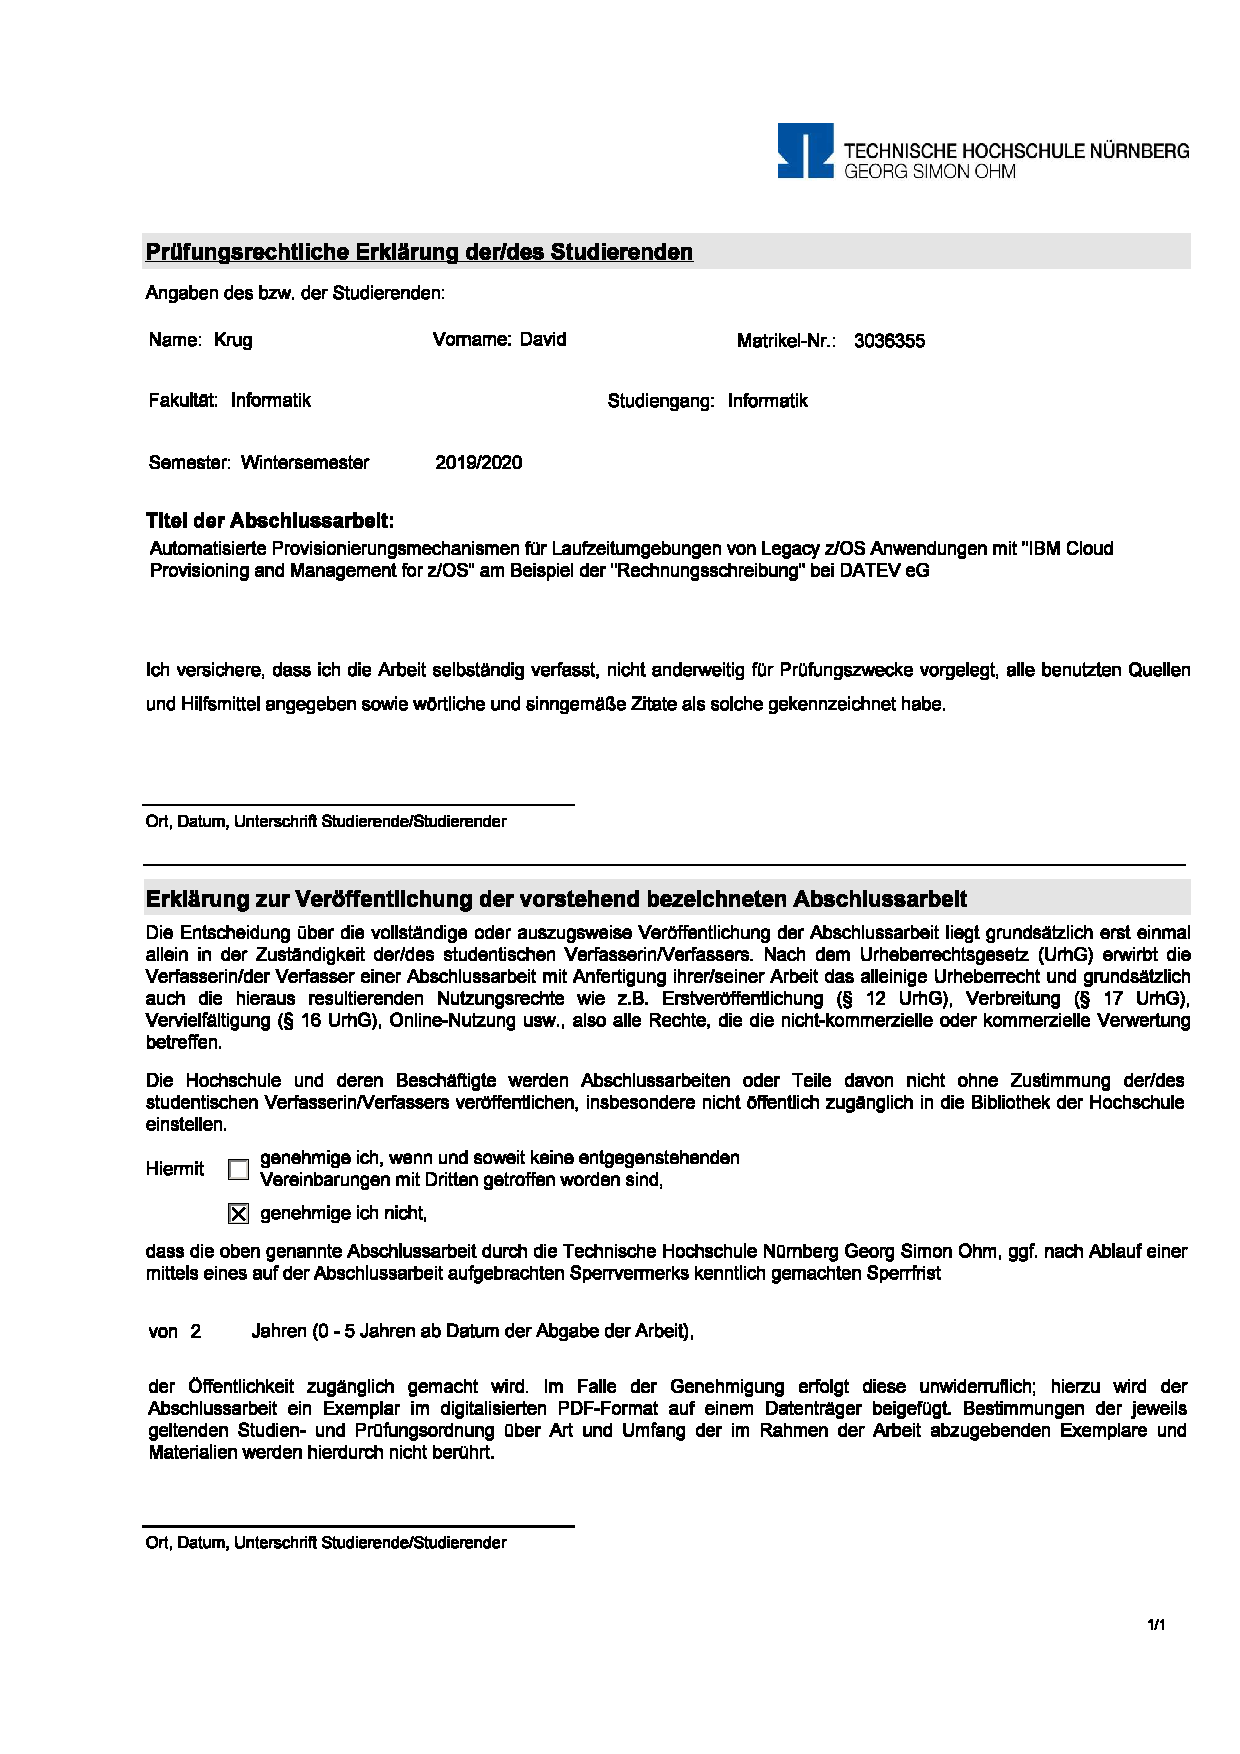
\includepdf{SB_0050_FO_Pruefungsrechtliche_Erklaerung_und_Erklaerung_zur_Veroeffentlichung_der_Abschlussarbeit_public.pdf}\cleardoublepage

\thispagestyle{empty}
\section*{Kurzdarstellung}
\label{sec:kurzdarstellung}
Ziel dieser Arbeit ist es, zu bestimmen, ob die Bereitstellung von Laufzeitumgebungen für legacy z/OS Anwendungen über einen cloud nativen, Platform-as-a-Service Ansatz bei DATEV e.G. möglich ist.
Es werden folgende Forschungsfragen gestellt:
\begin{itemize}
\item Ist es möglich, den Bereitstellungsprozess für z/OS Anwendung bei DATEV e.G. mit Hilfe des \glqq IBM Cloud Provisioning and Management for z/OS\grqq-Tools an cloud native Prozesse ("Self Service") anzunähern?
\item Erzeugt die Nutzung von \glqq IBM Cloud Provisioning and Management for z/OS\grqq{} einen Mehrwert bei den Stakeholdern, also den Entwicklerteams und den Administratorenteams?
\end{itemize}

Dafür wurde anhand einer Beispielanwendung von DATEV das Tool \glqq IBM Cloud Provisioning and Management for z/OS\grqq untersucht.
Es wurden zwei vorhandene Möglichkeiten aufgezeigt, eine davon implementiert.
Für ein Meinungsbild bezüglich  Mehrwertes und Akzeptanz des Tools, wurden Interviews mit Stakeholdern durchgeführt.
Diese Bild zeigt, dass in dem Tool eine Chance auf Verbesserung der aktuellen Prozesse gesehen wird.

Ergebnis war auch, dass die implementierte Variante nicht optimal für den Praxiseinsatz bei DATEV e.G. ist, aber eine wichtige Basis für die automatisierte Bereitstellung von Laufzeitumgebungen für z/OS Anwendungen darstellt.
Weiterführende Forschung könnte darauf aufbauend Variante zwei untersuchen und  Möglichkeiten einer weiteren, parxisgeeigneteren  Optimierung des z/OS Bereitstellungsprozesses aufzeigen.



\cleardoublepage

\tableofcontents

\mainmatter
Begriffe, die im Glossar erläutert werden, werden bei ihrem ersten Auftreten \textcolor{red}{rot} markiert.

\chapter{Einleitung}\label{ch:einleitung}
\glqq I recently predicted the last mainframe will be unplugged on March 15, 1996\grqq\footnote{\cite[S. 4]{Alsop.1993}} - ein in der Großrechner-Welt bekannt gewordenes Zitat.
Es handelt sich um eine 1993 getroffene Vorhersage, nämlich dass der letzte Mainframe, auch Großrechner genannt, am 15 März 1996 abgeschaltet werden würde.
Warum war diese Vorhersage falsch? 
Wieso wird sich im Jahre 2020 immer noch mit dieser Technologie beschäftigt? 
Und was genau ist ein Großrechner?

Kurz gesagt ist ein Großrechner\footnote{Beschreibung im Absatz \ref{sec:mainframe} zu finden} ein leistungsstarkes, zentralisiertes Serversystem.
In dieser Arbeit wird nur auf Mainframes aus dem Hause IBM, die sogenannte z-Plattform, eingegangen.
Damit ist auch der Technologiestack festgelegt.
Das verwendete Betriebssystem ist z/OS, darauf werden Middleware Produkte wie CICS\footnote{Anwendungsserver, CICS Beschreibung Absatz \ref{cics}}, das Datenbanksystem Db2\footnote{ Beschreibung Absatz \ref{sssec:db2}} sowie die Messaging Lösung \glqq IBM MQ\grqq{}\footnote{Beschreibung im Absatz \ref{sec:mq} zu finden} betrieben.
Als Programmiersprachen werden z.B. COBOL, IBM Assembler, C und C++ verwendet. 
Seit ca. 1997 ist auch Java auf dem Mainframe verfügbar. \footnote{\cite[S. 6]{Steegmans.2003}}.

Der IBM Mainframe hat eine lange Geschichte.
Vor mehr als fünfzig Jahren wurde der erste Großrechner, das sog. \glqq System/360\grqq{} vorgestellt.
Bis in die 90er Jahre spielte der IBM Mainframe eine Hauptrolle auf dem Computermarkt, dann gewannen zunehmend verteilte Client-Server-Systeme an Bedeutung.\footnote{\cite[Kap. 5]{Ceruzzi.2003}}
Seitdem gilt der Mainframe bereits als \glqq  legacy\grqq{} und damit als \glqq Altlast\grqq\footnote{\cite{.22.2.2020}}.

Wieso also wird sich mit der Mainframe Technologie noch beschäftigt? Eine Antwort: Auf dem Mainframe werden auch im Jahr 2020 geschäftskritische Anwendungen in der ganzen Welt gehostet.
So verwenden laut IBM 92 der 100 weltweit führenden Banken für ihre Kernabläufe einen IBM Mainframe.
Dies beinhaltet 87 Prozent aller Kreditkartentransaktionen und ca. 350.000 Transaktionen pro Sekunde.\footnote{\cite{.25.2.2020c}}
Inklusive dieser Transaktionen verarbeiten Großrechner heutzutage weltweit circa 1,2 Millionen CICS Transaktionen pro Sekunde.\footnote{\cite{.23.11.2019b}}
Im Vergleich hierzu werden 63.000 Google Suchanfragen pro Sekunde abgesetzt.  \footnote{\cite{.02.12.2019}}

Aus der Kombination von hohem Workload, der Abhängigkeit von einem Hersteller (IBM) und dem als veraltet geltenden Technologiestack entstehen jedoch zunehmend Risiken.
Es wird immer schwieriger, Nachwuchs in diesem Bereich zu finden.
Zum einem, da Mainframe-Know How kaum noch an Universitäten gelehrt wird.
Die Seite des Hochschulkompass\footnote{\cite{.09.02.2020}} liefert z.B. weder für \glqq Mainframe\grqq{} noch für \glqq Großrechner\grqq{} einen Treffer.
Zum anderen ist der demographische Faktor bei den Wissensträgern nicht zu vernachlässigen. Diese sind - wie die Technologien auf dem Mainframe - in die Jahre gekommen und erreichen das Rentenalter.\footnote{\cite{.25.2.2020f}}

Ein weiteres Problem ist, dass eine Firma, die einen IBM Großrechner mit z/OS betreibt, von dem oben genannten proprietären Technologiestack abhängig ist, dass heißt, es existiert eine starke Hersteller- und Plattformabhängigkeit, z.B. in Bezug auf CICS, Db2, IBM-COBOL-Compiler, IBM Assembler.

Offensichtlich betreiben dennoch etliche Firmen einen IBM Großrechner.
Dazu zählen hauptsächlich Banken, Versicherungen, Fluggesellschaften usw.\footnote{\cite{.25.2.2020c}}
Der gemeinsame Nenner dieser Unternehmen ist, dass sich über die Jahre und Jahrzehnte enorme Investitionen auf dem Mainframe angesammelt haben.
Die entstandenen, hochgradig geschäftskritischen Kernsysteme haben hohe Anforderungen an Massendatenverarbeitung, Sicherheitsstandards und Hochverfügbarkeit.
All diese Punkte sprechen nach wie vor für die Nutzung eines Großrechners, z.B. auch bei der DATEV e.G. (Kommentar: hier wäre ein Zitat schön, von einer Bank o.ä. ich schau mal ob ich was finde)

Die DATEV e.G. wurde am 14.02.1966 von 65 Steuerbevollmächtigen gegründet.
Sie verfolgten mit der Gründung das Ziel, Buchführungsaufgaben für ihre Mandanten mit Hilfe der neu aufkommenden EDV zu bewältigen.
Aufgrund hohen Mitgliederwachstums wurde hierfür bereits 1969 in einen firmeneigenen IBM-Großrechner investiert.\cite{.25.11.2019c}
Heute umfasst das Leistungsspektrum der DATEV e.G. unter anderem das Rechnungswesen, Personalwirtschaft, Consulting, IT-Sicherheit, Weiterbildung für ihre Kunden, in erster Linie Steuerberater, Wirtschaftsprüfer und Rechtsanwälte, und deren Mandanten.
Ein nicht unbeträchtlicher Teil dieser betriebswirtschaftlichen Anwendungen läuft bis heute ganz oder als Backend von Client-Anwendungen auf einem IBM Großrechner im DATEV Rechenzentrum.
So werden pro Tag circa 150.000 \Glspl{Batch-Job} und circa 90 Millionen CICS-Transaktionen verarbeitet.
Diese Last wird von circa 14.000 aktiven Modulen erzeugt.
Wie in der Abbildung \ref{fig:Programmiersprachen} zu sehen ist, ist COBOL mit circa 46\% Prozent die am häufigsten verwendete Programmiersprache am Großrechner bei der DATEV e.G..
Durch diese Module werden unter anderem im Monat circa 11 Millionen Lohnabrechnungen erstellt und circa eine Millionen Umsatzsteuer-Voranmeldungen durchgeführt. 
2018 wurde mit den DATEV Produkten erstmals die Umsatz-Milliarde erreicht.\footnote{\cite{.27.2.2020b}}

\begin{figure}
\begin{tikzpicture}
\begin{axis}[
             width=14cm,
             height=8cm,
             symbolic x coords={COBOL,IBM Assembler,C,Java, Sonstige},
             x tick label style={font=\small,text width=1.7cm,align=center},
             xtick=data,
             nodes near coords,
      	  nodes near coords align={vertical}, 
             ymin=0,
             ymax=65,
             ylabel=\%,
             ylabel style={rotate=-90},
             ybar,
             enlarge x limits=.2,
             bar width=45pt,
             ]
\addplot coordinates{(COBOL,46) (IBM Assembler,33) (C,13) (Java,2) (Sonstige,6)};
\end{axis}
\end{tikzpicture}
\centering
\caption{Anteil der verwendeten Programmiersprachen auf dem Mainframe bei DATEV eG in Prozent}
\label{fig:Programmiersprachen}
\end{figure}

\section{Problemstellung}\label{sec:probstell}
Im Jahre 2020 ist der größte Konkurrent für den Mainframe die Cloud.
Laut einer Vorhersage aus dem Jahr 2018\footnote{Statistik im Anhang \ref{app:itworkload}} soll im Jahre 2020 circa 79 Prozent des weltweiten Workloads in einer Cloud verarbeitet werden.
Für die Entwicklung von neuen Online-Anwendungen im cloud-native Stil wurde bei der DATEV e.G. eine Platform-as-a-Service (PaaS)-Lösung geschaffen und neue DevOps\footnote{Siehe Absatz \ref{sec:analysecloud}} Prozesse aufgebaut.
Dies ist im Cloud-Zeitalter nötig, um mit einer verbesserten Entwicklungseffizienz und neuen Architekturen Anwendungen (\glqq Apps\grqq) schneller auf den Markt bringen und auf Kundenanforderungen schneller reagieren zu können. Stichwort: Continuous Integration, Continuous Delivery (CI/CD)\footnote{Siehe Absatz \ref{sec:cicd}}.
Ein Baustein der effizientern Prozesse durch PaaS sind die sog. \glqq Self Services\grqq.
D.h., Entwicklerteams können sich über sog. \glqq Cloud Services\grqq, z.B. Datenbanken wie PostgreSQL, Mongo und Messaginglösungen wie Kafka entweder manuell über einen Marktplatz (siehe Abbildung \ref{fig:markt}) oder automatisiert per \glqq Build-Pipeline\grqq{} eine  Laufzeitumgebung für ihre Anwendung zusammenbauen.
\begin{figure}[h]
\centering
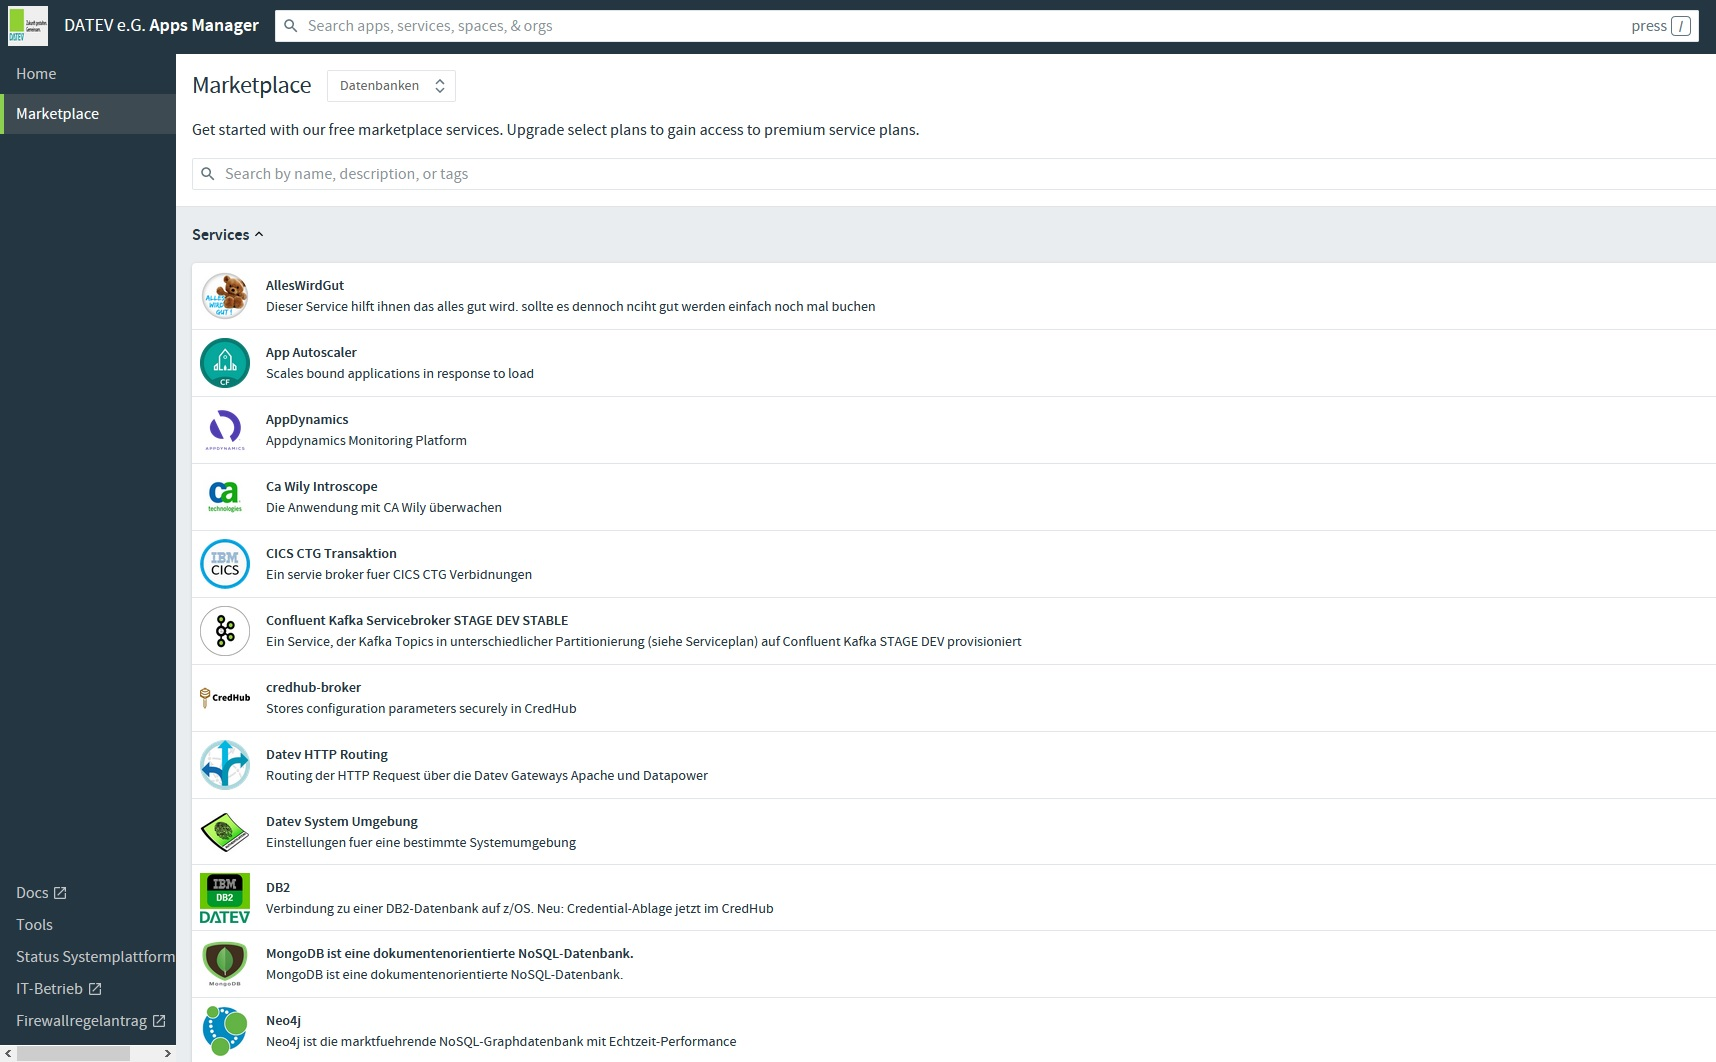
\includegraphics[width=\textwidth]{figures/CFMarketplace.jpg}
\caption{Cloud Foundry Marketplace bei DATEV e.G.}
\label{fig:markt}
\end{figure}
Eine genaue Beschreibung der Begrifflichkeiten erfolgt im Absatz \ref{sec:cloudnative}.
Den Entwicklern steht, neben modernen Entwicklungsumgebungen (IDE\footnote{Integrated Development Environment wie IntelliJ oder Eclipse}) und einer Sourceverwaltung mit Git, auch eine sog. \glqq Toolchain\grqq{} zur Verfügung. Diese beinhaltet Tools für Build, Test, Quality Gates und Deployment. 
Damit wird der Entwicklungsprozess automatisiert und man erhofft sich eine hohe Entwicklereffizienz. (Kommentar: hier würde ich nach wie vor die Grafik von unserem go/cloud Sharepoint mit einbinden)

Der Entwicklungsprozess für z/OS Anwendungen bei DATEV e.G. erscheint im Vergleich zu dieser PaaS-Lösung veraltet.
So wurde 2010 eine auf Eclipse basierende Entwicklungsumgebung für COBOL und IBM Assembler in der DATEV e.G. flächendeckend bereitgestellt.
Zuvor - und teilweise heute noch -  wurde mit Hilfe der in Abbildung \ref{fig:3270} gezeigten Oberfläche, dem sog. ISPF gearbeitet.
Diese stellte z.B. nur ein Syntaxhighlighting zur Verfügung.
\begin{figure}[h]
\centering
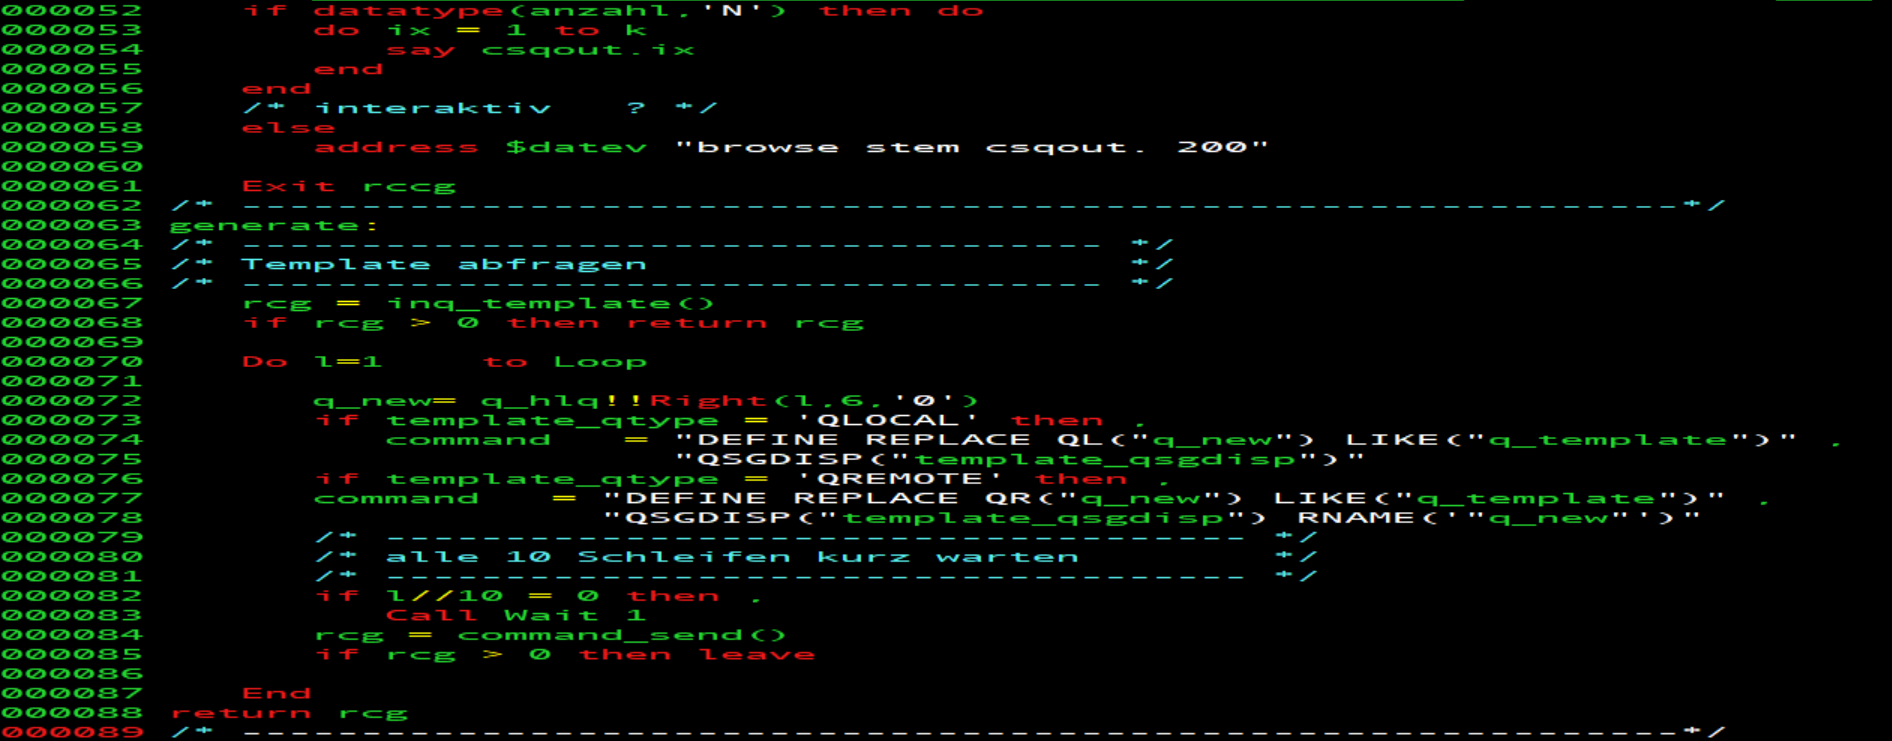
\includegraphics[width=\textwidth]{figures/rexxintso.png}
\caption{Auszug aus einem REXX Skript in der ISPF Oberfläche}
\label{fig:3270}
\end{figure}
Ein Meilenstein für die modernisierte z/OS Entwicklung bei DATEV war die Einführung von Git im Jahr 2018 auch für z/OS Sourcen. 
Dieses weit verbreitete Standard-Tool ist im z/OS Umfeld tatsächlich eine entscheidende Neuerung.
Dadurch wurde ein bis dato verwendetes eigenentwickeltes Tool für die Sourceverwaltung der z/OS Sourcen abgelöst.
Dieses stellte nur ein sehr einfaches Versionierungskonzept ohne aus Git bekannte Features wie Merge, Branch usw. bereit. 
Parallelentwicklung von verschiedenen Features war vorher mit viel Aufwand und Abstimmung möglich. 
Das Tooling wurde somit modernisiert, jedoch nicht der Entwicklungsprozess selbst.
Es teilen sich sehr viele Anwendungen die gleichen Entwicklungs-CICS/Db2/MQ Ressourcen.
Das heißt auch, dass eine Parallelentwicklung - trotz jetzt möglichen Git-Branches - an unterschiedlichen Features nur mit viel Abstimmungsaufwand und Absprachen innerhalb eines Entwicklungsteams, teilweise auch abteilungsübergreifend, möglich ist.
Werden Änderungen an bestehenden Ressourcen durchgeführt oder werden neue Systemumgebungen benötigt, entsteht weiterer Abstimmungsaufwand und weitere Absprachen.
Dadurch ist der aktuelle Prozess fehleranfällig und langsam.

Es bleibt die Frage, wie wird vor diesem Hintergrund mit den vielen Mainframebestandsanwendungen bei der DATEV e.G. in Zukunft umgegangen?
Die komplette Ablösung dieser Anwendungen durch cloud-native Lösungen ist eine Option, deren zeitlicher Rahmen und Machbarkeit aktuell nicht absehbar ist.\footnote{\ref{app:momappp} }
Für die Funktionsfähigkeit dieses Bestandsgeschäfts, das die Core-Business-Funktionalitäten der DATEV e.G. darstellt, muss also effiziente Weiterentwicklung und Wartung gewährleistet werden.
Auch im Falle einer geplanten Ablöse von Anwendungen muss je nach Strategie (z.B. \glqq Rewrite\grqq / \glqq Rearchitect\grqq)\footnote{(Kommentar, Strategiepatterns lt. Gartner, ich schick DIr enien Link)} das Alt-System parallel dazu über Jahre oder Jahrzehnte gepflegt und funktional aktuell gehalten werden.
Daraus folgt, dass aus Sicht der DATEV e.G. weiter in die IBM Mainframe Plattform investiert werden muss. 
Dies bedeutet Investitionen in die bereitgestellte Infrastruktur (Hardware, Betriebssysteme, Lizenzen), insbesondere aber auch Investitionen, die die oben genannten Anforderungen an Weiterentwicklung, Wartung und Entwicklungseffizienz sowie Effizienz im Betrieb adressieren.

\section{Ziel der Arbeit}\label{sec:ziel}
Es liegt also nahe, sich an den oben beschriebenen Prozessen zu cloud native Entwicklung zu orientieren. 
In diesem Zusammenhang läuft aktuell  bei DATEV e.G. ein Proof of Concept bezüglich automatisierter Builds von z/OS Anwendungen auf Basis von Jenkins basierten Pipelines. 
Dies ist auch die Voraussetzung für automatisierte Tests von z/OS Programmen im Rahmen des \glqq Continuous Integration, Continuous Deployment\grqq{} Ansatzes.
Was jedoch fehlt, sind \glqq Self Services\grqq{} für  Laufzeitumgebung und  Middleware.
Die dafür notwendige automatisierte Provisionierung einer z/OS Anwendungsumgebung, d.h Laufzeit, Middleware etc., ist aktuell noch weitgehend unerforscht. 
Hier sind die Prozesse bei DATEV und anderen Kunden oft noch proprietär, hoch spezialisiert,  manuell und nicht modernisiert. 
Gerade bei Mitarbeitern im Betrieb, die als Administratoren für die Middleware-Produkte arbeiten, sind die Bedenken groß, ob man diese Cloud-Vorgehensweise auf hochspezialisierte individuelle Komponenten wie CICS, DB2, IBM MQ anwenden kann, \glqq weil man so etwas bisher nicht vermisst hat\grqq\footnote{Marcel Amrein, IBM Senior Technical Sales Professional (MQ and CICS) (Quelle: Anhang \ref{app:ibm})}.
IBM bietet als eine Lösung \glqq IBM Cloud Provisioning and Management for z/OS\grqq{} an. 
Dies hat sich noch nicht flächendeckend durchgesetzt, aber \glqq Viele Kunden haben [...] im Moment Interesse, jedoch warten viele hier auf die ersten Erfahrungen von anderen\grqq\footnote{Tobias Leicher, IBM Senior IT Specialist for CICS and zAPI (Quelle: Anhang \ref{app:ibm})}.
Hier setzt diese Arbeit an und klärt folgende Fragen:

\begin{samepage}
\begin{itemize}
\item Ist es möglich, den Bereitstellungsprozess für z/OS Anwendung bei DATEV e.G. mit Hilfe des \glqq IBM Cloud Provisioning and Management for z/OS\grqq-Tools an cloud native Prozesse anzunähern?
\item Erzeugt die Nutzung von \glqq IBM Cloud Provisioning and Management for z/OS\grqq{} einen Mehrwert bei den Stakeholdern, also den Entwicklerteams und den Administratorenteams?
\end{itemize}
\end{samepage}

Um diese Fragen zu beantworten wird die Provisionierung einer z/OS Laufzeitumgebung für eine bestehende Anwendung untersucht.
Diese Anwendung sollte CICS als Anwendungsserver, eine Db2 Datenbank und IBM MQ als Messaginglösung nutzen, um für diese 3 Haupt-Technologien (Middleware-Komponenten) eine Aussage treffen zu können.
Die genaue Vorgehensweise wird im Kapitel \ref{ch:vorgehensweise} beschrieben.

\chapter{Motivation der DATEV e.G.}\label{ch:Firmenkontext}
Die in der Einleitung genannten Fragen werden aktuell im Rahmen des Querschnittsprojekts \glqq Mainframestrategie\grqq{} innerhalb der DATEV e.G. diskutiert. 
Der DATEV e.G. sind die zunehmenden Risiken durch schwierige Bereitstellung von Skills und der Herstellerabhänigkeit bewusst. 
Die Frage ist, wie wird mit den vielen Mainframebestandsanwendungen in Zukunft umgegangen?
Die komplette Ablösung dieser Anwendungen durch cloud-native Lösungen ist eine Option, deren zeitlicher Rahmen und Machbarkeit aktuell nicht absehbar ist.\footnote{\ref{app:momappp} }
Für die Funktionsfähigkeit dieses Bestandsgeschäfts, das die Core-Business-Funktionalitäten der DATEV eG darstellt, muss also effiziente Weiterentwicklung und Wartung gewährleistet werden.
Auch im Falle einer geplanten Ablöse von Anwendungen muss je nach Strategie (z.B. \glqq Rewrite\grqq / \glqq Rearchitect\grqq)\footnote{(Kommentar, Strategiepatterns lt. Gartner, ich schick DIr enien Link)} das Alt-System parallel dazu über Jahre oder Jahrzente gepflegt und funktional aktuell gehalten werden.
Daraus folgt, dass aus Sicht der DATEV e.G. weiter in die IBM Mainframe Plattform investiert werden muss. 
Dies bedeutet Investitionen in die bereitgestellte Infrastruktur (Hardware, Betriebssysteme, Lizenzen), aber insbesonders auch Investitionen, die die oben genannten Anforderungen an Weiterentwicklung, Wartung und Entwicklungseffizienz sowie Effizienz im Betrieb adressieren.

Diese Arbeit beschäftigt sich im Schwerpunkt mit den Aspekten der Entwicklungs- und Betriebseffizienz. 
Ziel ist es, diese zu steigern und eine Homogenisierung von Skills zwischen Mainframe-Entwicklern und Cloud-Entwicklern zu erreichen. 
Zur Entwicklungseffizienz gehört z.B. die in der Einleitung genannte moderne, auf eclipse basierende Entwicklungsumgebung ID/z (Kommentar, irgendwie verlinken auf Glossar o.ä.).
Diese wird bei DATEV eG schon seit ca. 10 Jahren firmenweit bereitgestellt.
Relativ neu (Seit 2018) ist die Nutzung von GIT als Sourceverwaltung für z/OS Artefakte. 
Dieses weit verbreitete Standard-Tool in der Cloud und Open Source Entwicklung ist im z/OS Umfeld tatsächlich eine entscheidende Neuerung. (KOmmentar: hier könnten wir ein Zitat von mir einfügen, dass ich über Konferenzteilnahmen andere Kunden kenne und deshalb weiß, wie schwer sich Mainframe-Kunden mit GIT tun). 
Aktuell (2019-2020) läuft bei DATEV e.G. ein Proof of Concept bezüglich automatisierter Builds auf Basis von Jenkins basierten Pipelines.
Dies ist auch die Voraussetzung für automatisierte Tests (Unit-Tests, Modul-Tests) von z/OS Programmen im Rahmen des \glqq Continuous Integration, Continuous Deployment\grqq{}\footnote{Beschreibung in Absatz \ref{Grundlagen}} Ansatzes.
Die dafür notwendige automatisierte Provisionierung einer z/OS Anwendungsumgebung, d.h Laufzeit, Middleware etc., um die gebauten Komponenten (COBOL, IBM Assembler-Programme) dann auch automatisiert testen zu können ist aktuell noch weitgehend unerforscht. 
Hier sind die Prozesse bei DATEV und anderen Kunden oft noch proprietär, hoch spezialisiert,  manuell und  nicht modernisiert. 
Gerade bei Mitarbeitern im Betrieb, die als Administratoren für die Middleware arbeiten, sind die Bedenken groß, ob man diese Cloud-Prozesse auf hochspezialisierte individuelle Komponenten wie CICS, DB2, IBM MQ anwenden kann.
Die von IBM hier angebotenen Lösungen, die durch das \glqq IBM Cloud Provisioning and Management for z/OS\grqq-Toolkit ermöglicht werden, haben sich noch nicht flächendeckend durchgesetzt, aber es herrscht Interesse an Erfahrungen und Einschätzungen.
Hier setzt diese Arbeit an und klärt die in der Einleitung genannten Fragen.



\chapter{Grundlagen}\label{ch:grundlagen}
In diesem Kapitel werden für diese Arbeit wichtige Begriffe erläutert.

\section{Mainframe / Großrechner}\label{sec:mainframe}
Mainframe und Großrechner werden in dieser Arbeit gleichbedeutend verwendet.
Im modernen Sprachgebrauch kann ein Großrechner als größte zur Verfügung stehende Serverart betrachtet werden.
Er wird von Unternehmen verwendet, um  kommerzielle Datenbanken, Transaktionsserver und Anwendungen, die einen hohen Grad an Sicherheit und Verfügbarkeit benötigten, zu hosten.
Im Gegensatz zu verteilten Serversystemen, bei denen die Funktionalitäten auf einzelne Server, wie zum Beispiel einen E-Mail-Server, einen Datenbank-Server, einen Web-Server usw. aufgeteilt sind, handelt es sich bei einem Mainframe um ein zentralisiertes System.
Unter anderem sind Datenbanksysteme und Anwendungsserver sogenannte \glqq Subsysteme\grqq.
\cite{Ebbers.2011}

\subsection{Batch}
Batch beziehungsweise Batch-Verarbeitung bezeichnet in der IT die sog. \glqq Stapelverarbeitung\grqq.
Das heißt, dass Programme mit minimalem menschlichen Eingreifen nacheinander abgearbeitet werden.
Dies geschieht meist zu einer vorher festgelegten Zeit, gesteuert wird dies über sog. \glqq Scheduling\grqq-Systeme.
Zum Beispiel wird einmal am Tag zu einer ganz bestimmten Uhrzeit die tägliche Bewertung\footnote{Beschreibung in Absatz \ref{sssec:täglbew}} der DATEV Rechnungsschreibung durchgeführt.
Die auszuführenden Programme laufen in sogenannten \glqq Batch-Jobs\grqq.
\cite{Ebbers.2011}

\subsection{Batch-Job / Job}\label{ssec:job}
In einem Batch-Job, in dieser Arbeit wird \glqq Job\grqq{} gleichbedeutend verwendet, wird dem System mitgeteilt welches Programm mit welchen Ein- und Ausgabedateien und Parametern gestartet werden soll.
Die Skriptsprache, die diese Jobs definiert, ist im IBM-Mainframe-Umfeld die sog. \glqq Job Control Language\grqq, kurz JCL.
Die drei Grundbausteine der JCL werden im Folgendem beschrieben.

Zunächst ist \glqq JOB\grqq{} zu nennen, auch Jobkarte genannt.
Hier wird der Name des Jobs, Berechnungsinformationen, maximal zur Verfügung stehende CPU-Zeit und weitere Job-weite Parameter gesetzt.
Im Beispiel \ref{fig:jclBsp} Zeilennummer eins bis drei.

Innerhalb eines Jobs wird mit Hilfe des \glqq EXEC\grqq{} Befehls dem System mitgeteilt, welches Programm gestartet werden soll.
Es können mehrere \glqq EXEC\grqq{}  Befehle in einem Job vorkommen, dabei wird jeder einzelne als sogenannter \glqq Job step\grqq{} bezeichnet.
Dabei können dem Programm neben den Ein-/Ausgabedateien auch weitere Parameter übergeben werden.
Im Beispiel \ref{fig:jclBsp} Zeilennummer zehn.

Als letztes ist der \glqq DD\grqq{} Baustein zu nennen.
\glqq DD\grqq{} steht für Data Definition.
Ein DD-Statement verknüpft den sog. DD-Namen mit einer Datei oder einem I/O Gerät und ist somit ein Alias für diese.
Ein \glqq DD\grqq{} Baustein ist immer an ein \glqq EXEC\grqq{} Befehl gebunden.
Einem \glqq EXEC\grqq{} können mehrere \glqq DD\grqq{} Bausteine zugeordnet sein. 
Im Beispiel \ref{fig:jclBsp} Zeilennummer 12 bis 15 und 19.
Hier ist auch zu sehen, dass Daten auch Inline an ein DD-Statement übergeben werden kann.
\cite{Ebbers.2011}

\begin{figure}[h]
\centering
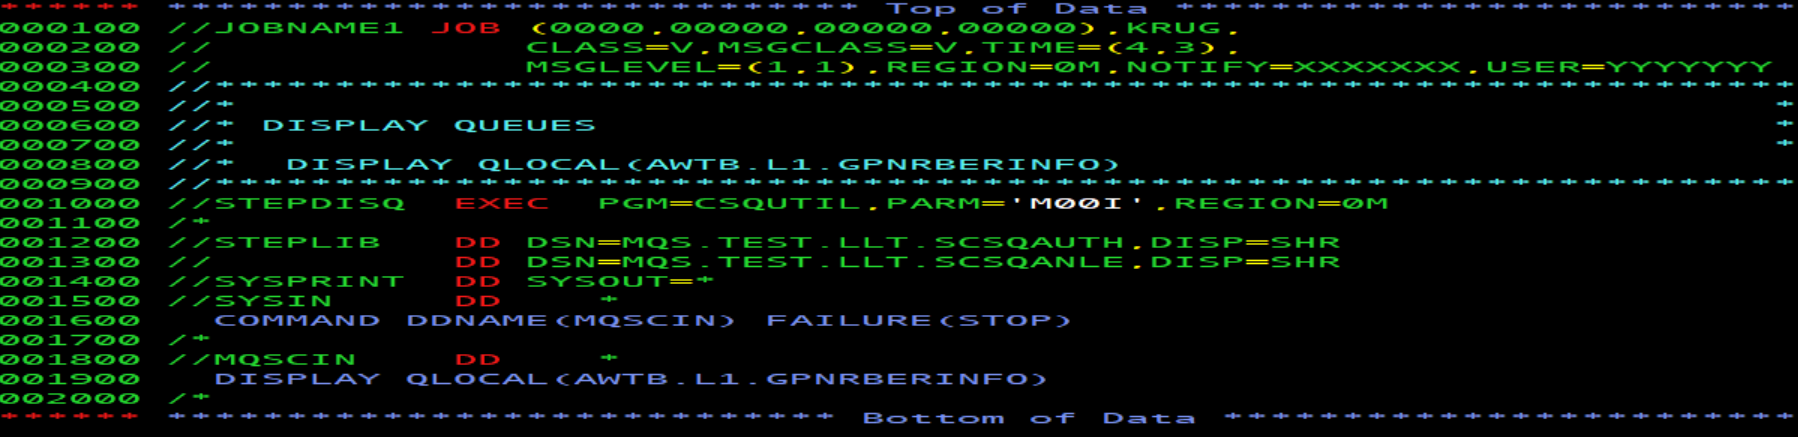
\includegraphics[width=\textwidth]{figures/dispq.PNG}
\caption{Job Beispiel, Display einer IBM MQ}
\label{fig:jclBsp}
\end{figure}

\subsection{Resource Access Control Facility}
Die Resource Access Control Facility, kurz RACF, ist ein externer Sicherheitsmanager für z/OS.
Dieser bietet eine Rechteverwaltung für das z/OS Betriebssystem an.
Damit werden unter anderem Zugriffsrechte auf Dateien und Subsysteme gesteuert.
\cite{InternationalBusinessMachinesCorporation.2008}

\subsection{REXX}
Die Restructures Extenden Executer Programmiersprache, kurz REXX, ist eine prozedurale Programmiersprache.
Die Sprache wird interpretiert.
Mittlerweile existieren jedoch auch REXX-Compiler.
\cite{Parziale.2007}

REXX versteht sich als Skriptsprache und kommt nicht nur am Mainframe zum Einsatz.
So kann es als Bindeglied für Betriebssystembefehle, grafischen Interfaces, Objekten, Funktionen und Serviceroutinen gesehen werden.
So wird es, wie auch in dieser Arbeit, unter anderem für die Automation von sich wiederholenden Systemadministrations Aufgaben eingesetzt.
\cite{Fosdick.2005}

\section{IBM Mainframe Architektur bei der DATEV eG}
Folgende Begriffe werden in diesem Absatz im Umfeld der DATEV eG erläutert:

\begin{samepage}
\begin{itemize}
\item Stages, Sysplexe und Logical Partitions
\item Middleware / Subsysteme
\item Architekturüberblick
\end{itemize}
\end{samepage}

Die DATEV eG bezogenen Informationen stammen aus Gesprächen mit Mitarbeitern der einzelnen Administratorenteams.

\subsection{Stages, Sysplexe und Logical Partitions}\label{sec:sysplex}
Innerhalb der DATEV eG existieren vier sogenannte \glqq Stages\grqq{} auf dem Mainframe.
Dabei handelt es sich um abgekapselte Systemumgebungen.
Eine Stage besteht aus einer oder mehreren \glqq Logical Partitions \grqq, kurz LPARs, mit eigenen Subsystemen und eigener Ressourcenverwaltung. 
Zu den Subsystemen zählen unter anderem CICS \footnote{Beschreibung in Absatz \ref{cics}},  Db2\footnote{Beschreibung in Absatz \ref{sssec:db2}} und IBM MQ\footnote{Beschreibung in Absatz \ref{sec:mq}}.
Dadurch wird eine strickte Trennung zwischen den Stages realisiert.
Die vier Stages werden im Folgenden beschrieben.

\subparagraph{\glqq Entwicklung\grqq}~\\
Stage auf der alle z/OS Entwickler an neuen Features arbeiten und erste kleinere Tests durchführen.

\subparagraph{\glqq Qualitätssicherung\grqq} ~\\
Hier werden vor allem Integrationstests mit extra dafür erstellen Testdaten durchgeführt.

\subparagraph{\glqq Vorproduktion\grqq}~\\
Die Vorproduktion steht für weitere Integrationstests zur Verfügung.
Jedoch produktionsnäher und auch mit Echtdaten, also Daten aus der Produktion.

\subparagraph{\glqq Produktion\grqq}~\\
Hier befindet sich die Software, die von den Kunden verwendet wird.
Ein Programm muss die Entwicklungs-, Qualitätssicherungs- und Vorproduktionsstages durchlaufen bevor es dem Kunden in der Produktion zur Verfügung gestellt wird.

Die LPARs der vier Stages sind auf zwei sogenannte  \glqq Sysplexe\grqq{} aufgeteilt.
Ein Sysplex kümmert sich um die Kommunikation zwischen den LPARs der einzelnen Stages und verwaltet Ressourcen LPAR übergreifend.
\cite{Kyne.2016}

Neben den oben erwähnten zwei Sysplexen existiert noch ein weiterer Sysplex.
Diese werden alle im Folgenden beschrieben.

\subparagraph{\glqq LAB/Test-Plex\grqq}~\\
Der Test-Plex ist als Labor für Änderungen am System zu betrachten.
So werden zum Beispiel neue Betriebssystemsversionen auf diesem geprüft.

\subparagraph{\glqq QS-Plex\grqq}~\\
Enthält unter anderem die LPARs der Entwicklung und der Qualitätssicherung.

\subparagraph{\glqq Prod-Plex\grqq}~\\
Im Prod-Plex sind die LPARs der Vorproduktion und der Produktion enthalten.

\subsection{Middleware / Subsysteme}
In diesem Absatz wird die verwendete Middleware beziehungsweise die verwendeten Subsysteme beschrieben.
Diese setzen auf dem IBM Mainframe Betriebssystem z/OS auf.

\subsubsection{Customer Information Control System}\label{cics}
Das Customer Information Control System, kurz CICS, ist ein Applikationsserver für einen IBM-Großrechner mit Betriebssystem z/OS und damit eine IBM Middleware.
Ein Applikationsserver stellt eine Umgebung zur Verfügung, in der Anwendungen gehostet werden können.
Dabei kümmert sich dieser unter anderem um Transaktionalität, Webkommunikation und Sicherheit.
Hierfür stellen Applikationsserver eine API zur Verfügung.
CICS hat einen Vorteil gegenüber anderen Anwendungsservern, es unterstützt verschiedene Programmiersprachen.
CICS ist ein Multi-Language Application Server und unterstützt z.B. COBOL, Assembler, Java und PLI.
So können Programme innerhalb einer Anwendung in der für ihren Use-Case am besten geeigneten Sprache implementiert werden.
\cite{Rayns.2011}

Das CICS Subsystem einer Stage umfasst mehrere CICS Instanzen.

\paragraph{CICS Instanz} ~\\
Unter einer CICS Instanz ist ein einzelner Bereich, der auf dem z/OS Kernel aufsetzt, zu verstehen.
Dieser Bereich ist mittels einer eindeutigen CICS ApplicationID gekennzeichnet und kann darüber explizit angesprochen werden.
Eine CICS Instanz verwaltet mehrere CICS Transaktionen.

Wenn in dieser Arbeit von dem CICS gesprochen wird, ist die CICS-Instanz damit gemeint.

\paragraph{CICS Transaktion}\label{subsec:trans} ~\\
Ein Businessablauf wird im CICS in einer Transaktion gekapselt.
Eine Transaktion kann mehrere Programme unterschiedlicher Programmiersprachen umfassen und wird über eine eindeutige \glqq TransaktionsID\grqq{} identifiziert..

Über die TransaktionsID wird der Ablauf gestartet.
Dies kann sowohl per Webanfrage oder per Messaging Queue als auch aus einem anderen Programm heraus oder manuell geschehen.
In der Transaktion werden alle Änderungen, die Programme an Ressourcen, wie zum Beispiel einer Datenbank oder Dateien tätigen, protokolliert.
So wird im Fehlerfall die Möglichkeit eines Rollbacks sichergestellt.
 \cite{Rayns.2011}

\paragraph{Voraussetzungen}\label{subsec:voraus} ~\\
Bei der DATEV eG kümmert sich ein Team, die \glqq CICS Administration\grqq{} um das Erstellen einer CICS-Instanz, starten dieser Instanz und ist generell für alles rund um die Administration des CICS Transactions Servers zuständig.
Der Fokus dieser Arbeit liegt auf dem Erstellen (\glqq Provisionieren\grqq{}) einer CICS-Instanz. Es werden nur die dafür notwendigen Voraussetzungen dargelegt.
Außerdem liegt der Fokus auf Entwicklungs-CICS-Systemen, auf der sog. Entwicklungs-Stage, nicht auf den produktiven CICS-Systemen der DATEV eG. 
Aus diesem Grund werden nur Schritte, die für ein solches Testsystem benötigt werden, dargestellt.
Eine weitere Rahmenbedingung besteht darin, dass nur die Arbeitsschritte, die mit z/OSMF\footnote{Beschreibung in Absatz \ref{sec:zosmf}} automatisiert werden, erläutert werden.

\paragraph{Einrichtung CICS Instanz}\label{subsec:createCICS}~\\
Die in diesem Absatz benötigten Informationen stammen aus Gesprächen mit Mitarbeiter 2 aus der Abteilung, die für die CICS Administration zuständig ist.
Um eine lauffähige CICS Instanz den Vorausetzungen aus dem Absatz \ref{subsec:voraus} entsprechend einzurichten, sind mehrere Schritte notwendig.
Diese werden im Folgendem beschrieben.

\subparagraph{CICS spezifische Dateien}\label{sssec:speziDat} ~\\
Zunächst müssen CICS spezifische Dateien im z/OS angelegt werden.
Im Fall des dieser Arbeit zugrunde liegende Beispiels handelt es sich um 17 verschiedene VSAM\footnote{Virtual Storage Access Method, spezielle Dateiart, die schnelle I/O-Zugriffe ermöglicht.\cite{Lovelace.2013}} Dateien.
Diese Dateien benötigt die CICS Instanz um zum Beispiel Systemfehler zu protokollieren oder den Debugger aktivieren zu können.

\subparagraph{CSD} ~\\
In der Datei \glqq CICS System Defintion\grqq, kurz CSD, muss jede Ressource, die dem System zur Verfügung stehen soll, definiert werden.
Eine CSD Datei kann für mehrere CICS Instanzen verwendet werden.
Eine CSD Datei besteht aus mehreren Einträgen.
Ein Eintrag besteht aus einer Gruppe und einer Liste.
Die Gruppe ist hierbei die Definition einer Systemressource und muss manuell angelegt werden.
Bei der Liste handelt es sich um das System, welches diese Ressource benötigt.
Dort ist unter anderem für jede CICS Instanz hinterlegt, zu welchem Db2 Datenbanksystem und welchem IBM MQ Messagingsystem sich diese Instanz verbinden soll.

\subparagraph{STC Job} ~\\
Bei einem Started Task Control-Job, kurz STC Job, handelt es sich um einen Batch Job, der mit Hilfe des \glqq START\grqq-Konsolenkommandos innerhalb von z/OS gestartet werden kann.
Dieser Batch Job wird deshalb auch als Started Task bezeichnet.\cite{Cassier.2007}
Bei der DATEV eG existiert für jede Instanz eines Subsystems ein solcher Job, so also auch für CICS.
In diesem werden zunächst einige zur Laufzeit benötigten Bibliotheken und Dateien eingebunden, unter anderem die CICS spezifischen Dateien\footnote{Beschreibung in Absatz \ref{sssec:speziDat}}.
Außerdem werden hier die SIT \footnote{CICS system initialization table} Parameter definiert.
Zunächst wird festgelegt welche Standard SIT verwendet werden soll.
Anschließend können diese Standardwerte überschrieben werden.
Zu diesen Parameter zählen unter anderem der eindeutige Name der CICS Instanz, der Speicherort der dazugehören CSD und die Information, ob eine Verbindung zu einem Db2 Datenbanksystem hergestellt werden soll.

\paragraph{Entfernung CICS Instanz} ~\\
Um eine CICS Instanz zu entfernen muss diese zunächst gestoppt werden.
Dies ist über das \glqq STOP\grqq-Konsolenkommando von z/OS möglich.
Anschließend müssen alle im Absatz \ref{subsec:createCICS} beschriebene Schritte rückgängig gemacht werden.
Also müssen die für diese Instanz spezifischen Dateien, die Einträge für die CICS Instanz aus der CSD Datei und schließlich auch der STC Job gelöscht werden.

\subsubsection{Db2}\label{sssec:db2}
Db2 ist ein relationales Datenbanksystem, welches unter anderem als Subsystem eines z/OS Betriebssystems läuft.
Einer Stage können mehrere Datenbanksysteme, auch Instanz genannt, zugeordnet werden.
In diesem befinden sich die Datenbanken und Tabellen.

\subsubsection{IBM MQ}\label{sec:mq}
IBM MQ ist eine Messaging-Lösung der IBM.
Diese ermöglicht den asynchronen Datenaustausch zwischen Anwendungen mittels sogenannter Queues.
Alle IBM MQ Begrifflichkeiten, die in dieser Arbeit verwendet werden, werden im Folgenden erläutert.
\cite{Aranha.2013}

Das IBM MQ Subsystem einer Stage setzt sich aus einem oder mehreren Queue Managern zusammen.
Ein Queue Manager kann so als IBM MQ Instanz gesehen werden.

\paragraph{Queue Manager}~\\
Bei einem Queue Manager handelt es sich um die zentrale Ressource eines IBM MQ Systems.
Er verwaltet  alle anderen IBM MQ Ressourcen.
Dazu gehören unter anderem die Speichersteuerung der Daten und die Wiederherstellung dieser im Falle eines Fehlers.
Desweiteren koordiniert er den Zugriff aller Anwendungen auf die Nachrichten in den von ihm verwalteten Queues.
Um hierbei die Konsistenz sicherzustellen, sorgt er für Locking und die notwendige Isolation der Queues.
\cite{Aranha.2013}

\paragraph{Queues}~\\
In Queues werden die Nachrichten, die von Programmen gesendet und gelesen werden gespeichert.
Es gibt verschiedene Arten von Queues, die im Kontext dieser Arbeit relevanten Queues sind folgende:

\subparagraph{Die Local Queue.}~\\
Dabei handelt es sich um die einzige Queue Art, bei der die Nachrichten physikalisch gespeichert werden.
Die anderen Queue Arten nutzen als Basis immer eine Local Queue.

\subparagraph{Initiation Queue}~\\
Die sogenannte \glqq Initiation Queue\grqq{} ist eine spezielle Art der Local Queue.
Diese dient dem Queue Manager dazu, um unter bestimmten Bedingungen eine Trigger-Nachricht darauf zu schreiben.
So kann eine andere Local Queue so definiert sein, dass sobald eine Nachricht auf sie geschrieben wird eine solche Trigger-Nachricht erzeugt wird.
Dies ermöglicht, dass Anwendungen nur starten, wenn wirklich Daten zum Verarbeiten vorhanden sind.
\cite{Aranha.2013}

\paragraph{Process}~\\
Für das Auslösen von Anwendungen wird nicht nur die Initiation Queue benötigt, sondern auch sogenannte \glqq Processes\grqq.
So muss der Local Queue, die den Start einer Anwendung auslösen soll, bei der Definition nicht nur die Initiation Queue bekannt gemacht werden, sondern auch ein Process.
Ein Process legt den \glqq Type\grqq{} und den Namen der zu startenden Anwendung fest.
Als \glqq Type\grqq{} können beispielhaft CICS oder auch WINDOWSNT für Windows unterstütze Platformen genannt werden.
Ist der \glqq Type\grqq{} CICS,  muss der Name der Transaktion angegeben werden, für Windows Platformen der Dateipfad der auszuführenden exe.
\cite{Aranha.2013}

\subsection{Architekturüberblick}
In Abbildung \ref{fig:archüber} sind die einzelnen Subsysteme mit ihren Instanzen dargestellt.
Als Grundbaustein dient allen der z/OS Kernel.

\begin{figure}[h]
\centering
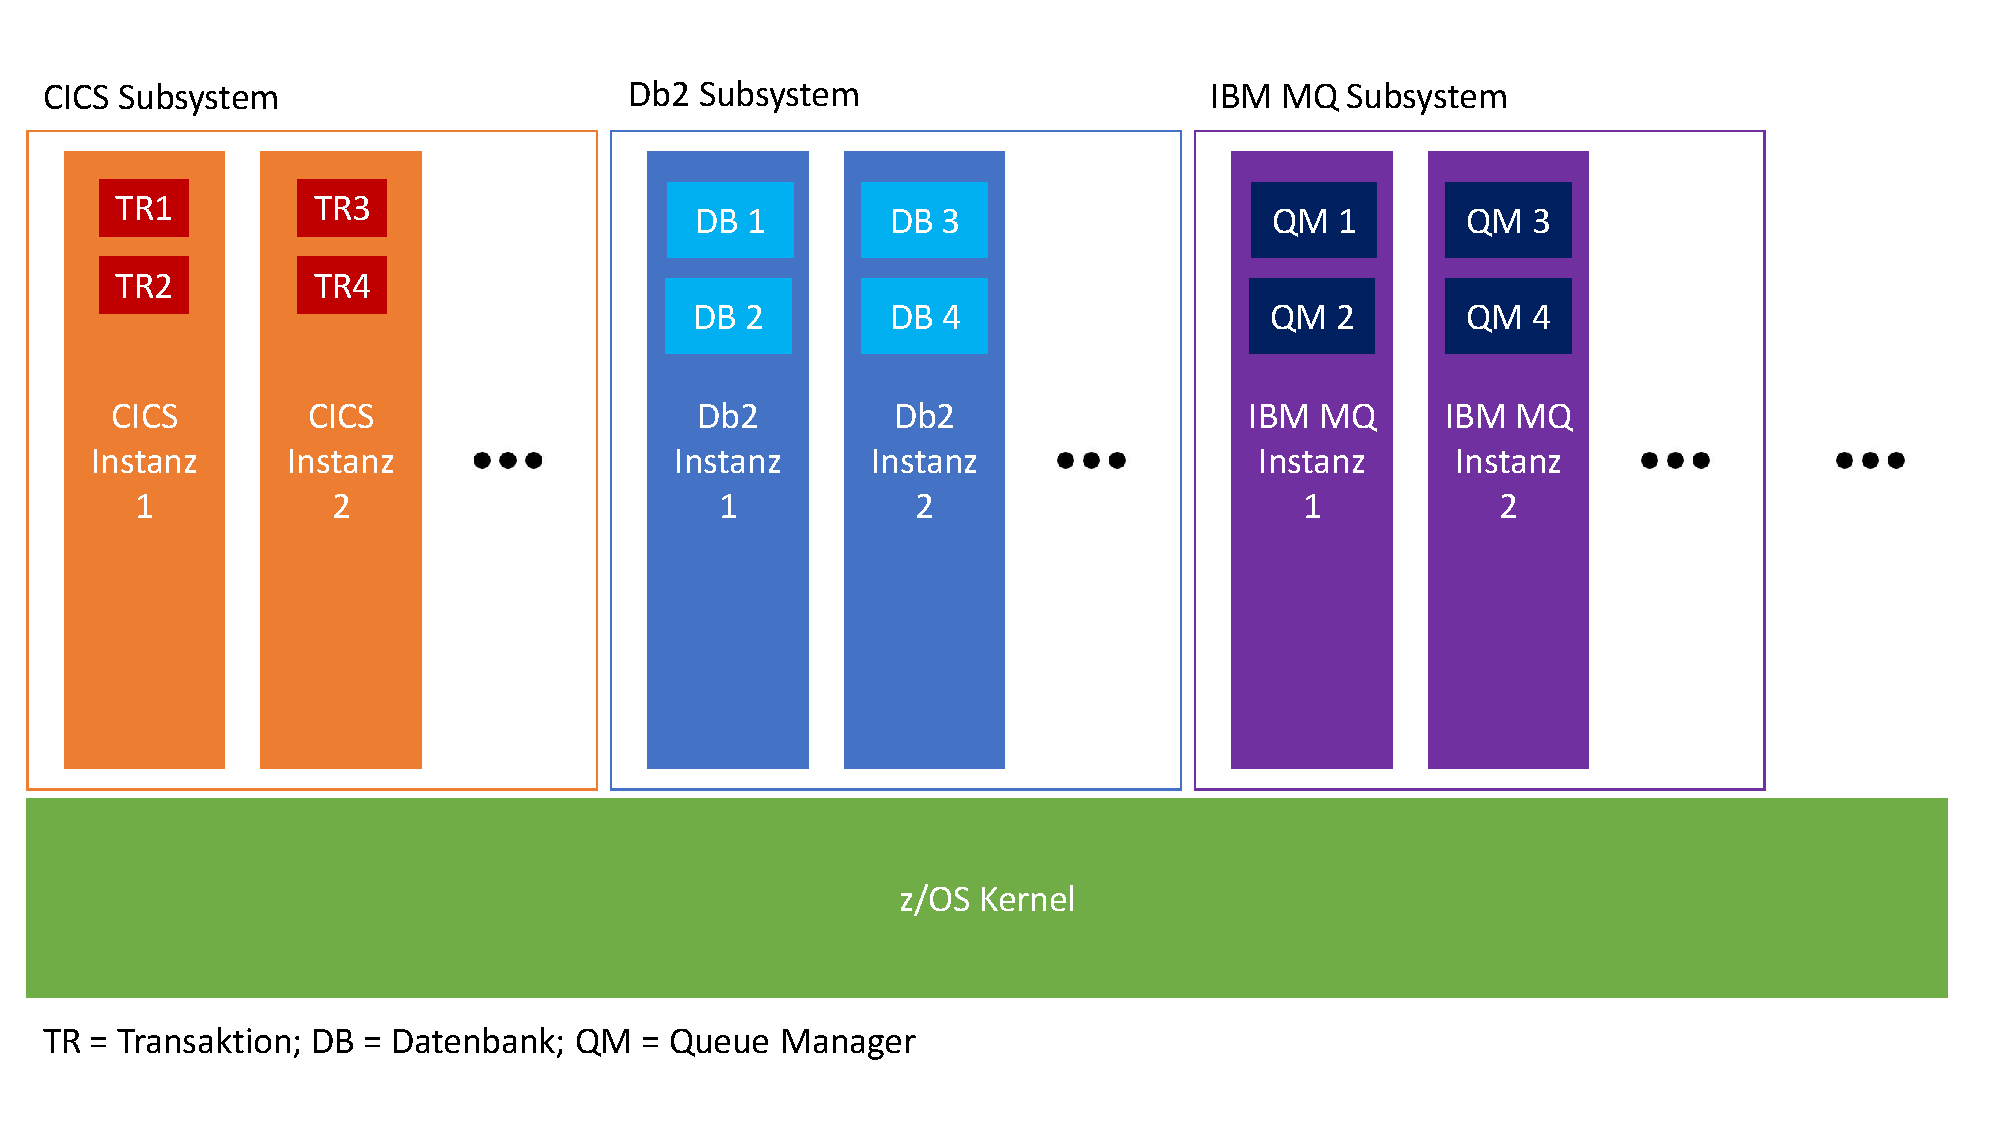
\includegraphics[width=\textwidth]{figures/architektur.pdf}
\caption{Architekturübersicht über die Subsysteme bei DATEV eG}
\label{fig:archüber}
\end{figure}

\section{IBM Cloud Provisioning and Management for z/OS}\label{sec:zosmf}
In diesem Absatz wird zunächst auf die für dieses Kapitel grundlegenden Begriffe eingegangen.
Das IBM Cloud Provisioning and Management for z/OS bietet die Möglichkeit, mehrere Systeme (sog. Middleware) innerhalb eines z/OS Betriebssystems zu provisionieren, unter anderem Laufzeitumgebungen wie CICS. 
Für diese Aufgaben stehen zwei Schnittstellen zur Verfügung.
Zum einen das z/OS Provisioning Toolkit, (z/OSPT) und zum anderen z/OS Management Facility (z/OSMF).
\cite{KeithWinnardGaryPuchkoffHirenShah.2016}

\subsection{Begrifferklärung}
Im Folgenden werden einige allgemeine Begriffe, die im Umfeld des Tools \glqq IBM Cloud Provisioning and Management for z/OS\grqq{} vorkommen, erläutert.

\subsubsection{Provisioning}
Ins Deutsche übersetzt bedeutet es Bereitstellung, in dieser Arbeit wird auch Provisionierung verwendet.
In dieser Arbeit umfasst dieser Begriff die Bereitstellung einer Laufzeitumgebung, beziehungsweise den Prozess, der hierfür benötigt wird.

\subsubsection{Workflow}\label{sssec:workflow}
Ein Workflow ist eine beliebig komplexe, eindeutige Aneinanderreihung von sogenannten Steps.
Nach der Ausführung dieser Steps wird ein bestimmtes Ziel erreicht, zum Beispiel die erfolgreiche Bereitstellung eines CICS Systems.
Für die Definition eines Workflows, der dazugehörigen Steps und ihrer Variablen wird XML genutzt.
Ein Step beschreibt einen Teilablauf eines Workflows.
Innerhalb eines Steps können sowohl interne und externe Scripte als auch JCLs und somit Programme ausgeführt werden.
Darüber hinaus besteht die Möglichkeit REST-Calls auszuführen.
Es können Bedingungen für die Durchführung eines Steps definiert werden.
So ist es zum Beispiel möglich, einen Step nur durchzuführen, wenn eine bestimmte Variable einen bestimmten Wert besitzt.
Es wird ein XML Schema verwendet um sicherzustellen, dass in dem XML-Skript zur Laufzeit keine syntaktischen Fehler vorhanden sind.
\cite{Rotthove.2018}

Ein Nachteil von Workflows ist, dass diese statisch sind, das heißt, dass die Variablenzuweisungen immer zum Zeitpunkt der Erstellung stattfindet.
Dadurch ergibt sich, dass für jede kleine Änderung ein eigener Workflow erzeugt werden muss.
Somit ist ein Workflow eher ein Einmal- bzw. Wegwerfprodukt.

\subsubsection{Template}
Bei dem Nachteil von Workflows als Wegwerfprodukt setzen die sogenannten Templates an.
Ein Template besteht aus drei Dateien.

\begin{enumerate}
\item Datei für Eingabevariablen.\\
In dieser Datei kann Workflowvariablen Werte zugewiesen werden.
Diese Variablen müssen bei ihrer Definition im Workflow entsprechend gekennzeichnet sein.

\item Die sogenannte Aktion-Definitions-Datei.\\
Hier werden die Aktionen, die ein Anwender mit diesem Template durchführen kann, festgelegt.
Einer Aktion wird eine Workflow Definitions Datei und somit ein Workflow zugewiesen.
Darin ist die Datei für die Eingabevariablen und die Festlegung, welche Variablen davon verwendet werden, anzugeben.

\item Die Manifest-Datei.\\
In dieser wird dem Template mitgeteilt, an welchem Speicherort sich die oben genannten Dateien befinden.
Da ein Template immer provisioniert werden kann, wird hier auch der Speicherort des Bereitstellungsworkflows angeben.
Zusätzlich kann noch eine Beschreibung des Templates hinzugefügt werden.
\end{enumerate}

Somit bildet ein Template einen Rahmen um mehrere Workflows und ermöglich eine schnellere De-/provisionierung.
Das hat den Vorteil, dass Variablen nur an einer Stelle geändert werden.
Daüber hinaus besteht die Möglichkeit, per Awendereingabe den Variablen zum Zeitpunkt der Provisionierung einen Wert zuzuweisen.
Somit ist ein Template deutlich flexibler als ein Workflow.
\cite{IBM.2019}

\subsubsection{Instance}\label{sssec:instance}
Hierbei handelt es ich um das Ergebnis nach der Provisionierung eines Templates, zum Beispiel um ein funktionsfähiges CICS.
Als Abgrenzung zu einer Instanz eines Subsystems, kann eine Template Instance auch Instanzen mehrer Subsystemen enthalten.

\subsection{z/OS Provisioning Toolkit}\label{sssec:zospt}
z/OSPT bietet ein Kommandozeileninterface für die Bereitstellung und das Verwalten von Laufzeitumgebungen.
In Abbildung \ref{fig:zospt_help} werden die möglichen Kommandozeilenbefehle mittels des Befehls \glqq zospt -h\grqq{} in einem Kommandofenster angezeigt.
\begin{figure}[h]
	\centering
	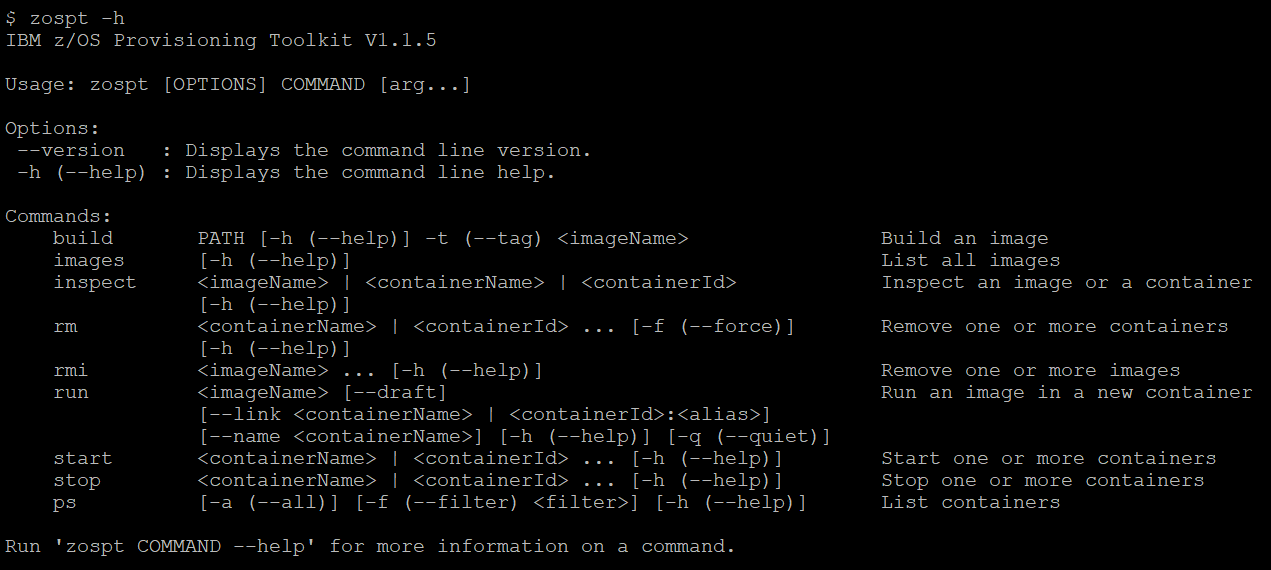
\includegraphics[width=\textwidth]{figures/zospt_help_putty.png}
	\caption{z/OSPT mögliche Kommandozeilenbefehle}
	\label{fig:zospt_help}
\end{figure}
Mit z/OSPT werden noch zwei weitere Begriffe eingeführt.\\
\glqq Images\grqq{}.
Dabei handelt es sich grundsätzlich um ein Template, jedoch kann dieses Template über eine weitere Inputdatei verändert werden.
Dadurch kann ein Template mit spezifischen Änderungen provisioniert werden, ohne dass ein neues Template erzeugt werden muss.
Dies erhöht die Flexibilität der Templates weiter.

\glqq Container\grqq{}.
Dabei handelt es sich eins zu eins um eine \glqq Instance\grqq \footnote{Beschreibung in Absatz \ref{sssec:instance}}.
\cite{IBM.2019b}

\subsection{z/OS Management Facility}\label{sssec:zosmf}
Der Hauptaugenmerk dieser Arbeit liegt  bei z/OSMF, da damit die Verwaltung von Workflows und Templates über eine browserbasierende Schnittstelle möglich ist.
Durch diese Oberfläche, in Abbildung \ref{fig:zosmf_welcome} dargestellt, ist es einfacher zu bedienen als das Kommandozeileninterface von z/OSPT  und somit wird der Einstieg in die Provisionierung erleichtert.

\begin{figure}[h]
\centering
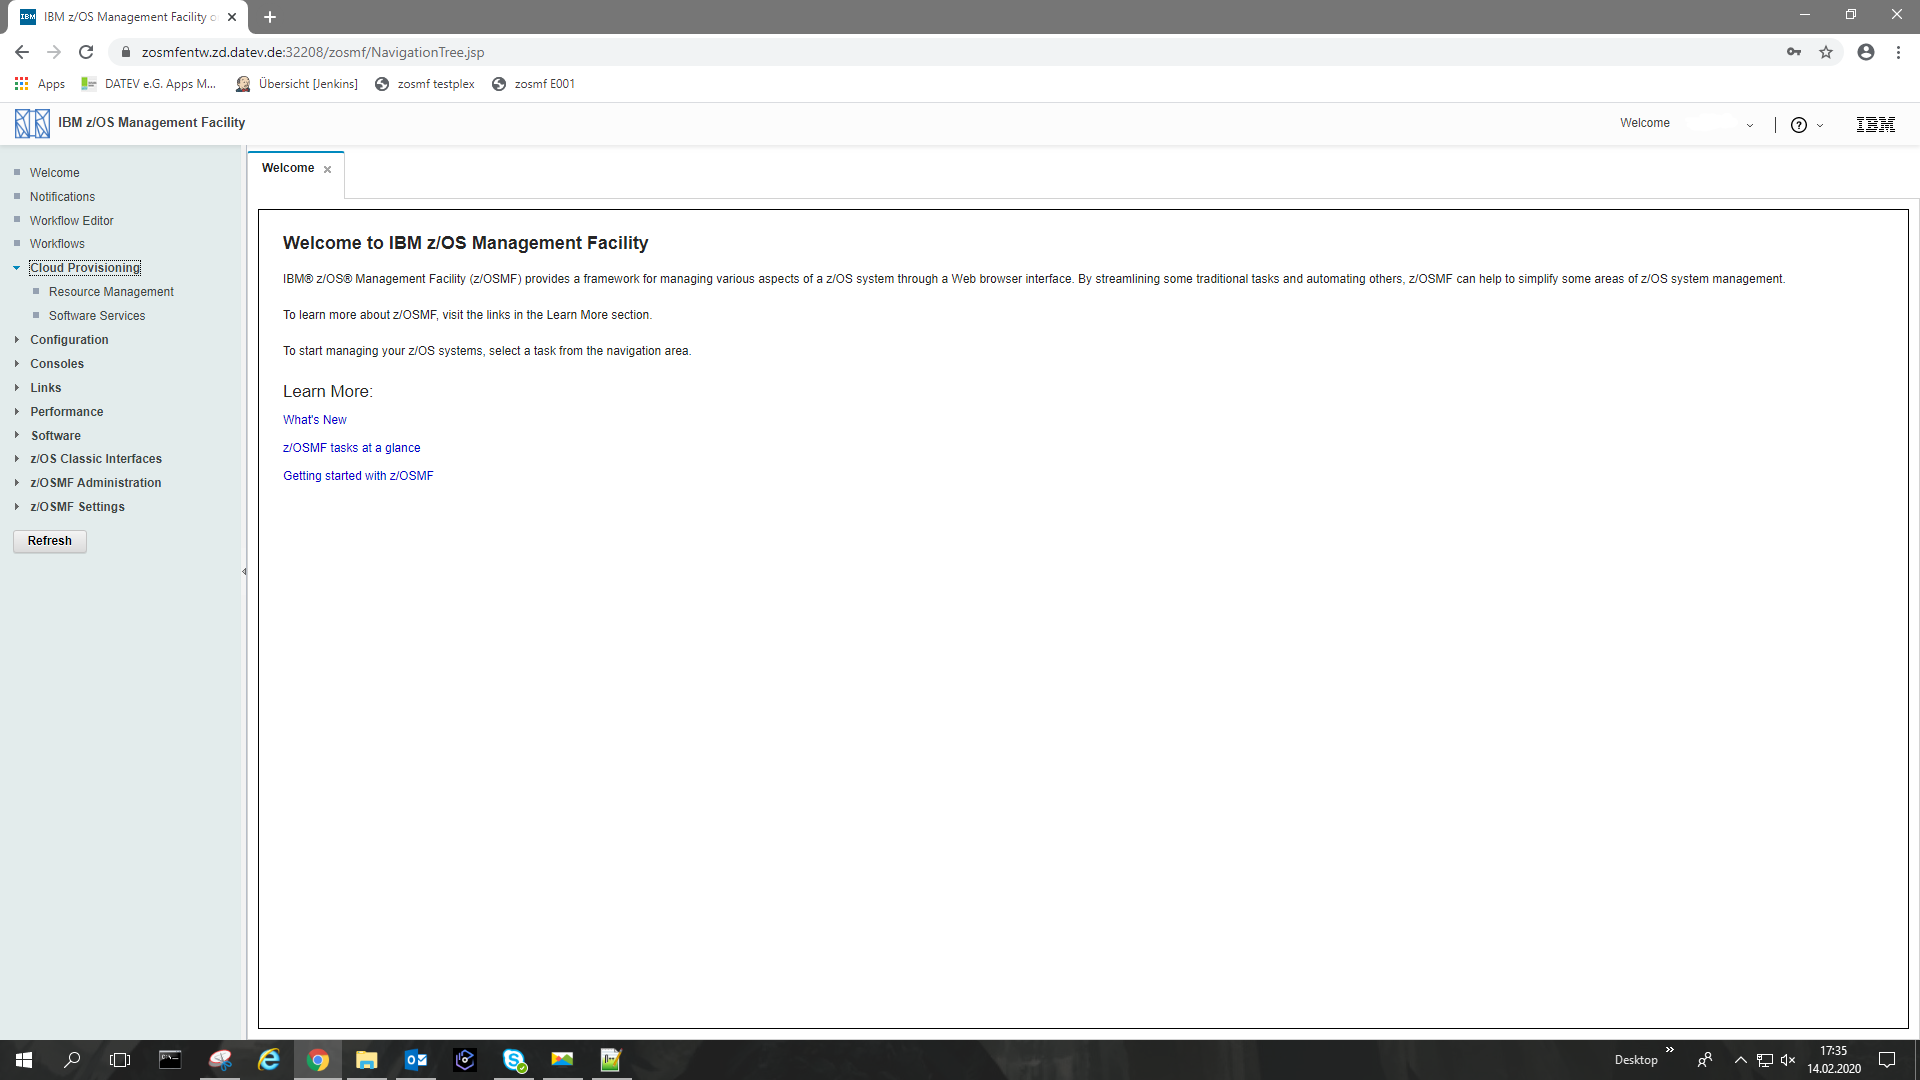
\includegraphics[width=\textwidth]{figures/zosmf.png}
\caption{z/OSMF Willkomens Ansicht}
\label{fig:zosmf_welcome}
\end{figure}

Die linke Seite der Abbildung \ref{fig:zosmf_welcome} zeigt den Umfang der z/OSMF  Funktionen.
Für diese Arbeit besitzt nur der Menüpunkt \glqq Cloud Provisioning\grqq{} Relevanz.
Unter diesem Punkt sind die Funktionalitäten für die automatisierte Bereitstellung von Templates zu finden.
\cite{Rotthove.2018}

Zuerst ist das \glqq Resource Management\grqq{} zu nennen..
Darunter werden sogenannte \glqq Domains\grqq{} und die dazugehörigen \glqq Tenants\grqq{} verwaltet.
Unter einer \glqq Domain\grqq{} ist ein System zu verstehen, das Systemressourcen in Ressourcenpools gliedert.
\glqq Tenants\grqq{} sind die dazugehörigen Rechtegruppen, die dem Anwender den Zugriff auf und die Nutzung von zugeordneten Templates ermöglicht.
Einem Template muss sowohl eine\glqq Domain\grqq{} als auch ein \glqq Tenant\grqq{} zugewiesen werden.
\cite{Rotthove.2018}

Zur Verwaltung der Templates und Instances kommen die \glqq Software Services\grqq{} zum Einsatz.
Dort können neue Templates über die \glqq Manifest Datei\grqq{} hinzugefügt werden.
Dann muss, wie oben beschrieben, eine \glqq Domain\grqq{} und ein \glqq Tenant\grqq{} zugwiesen werden.
Anschließend kann das Template, falls es keine Fehler beinhaltet, veröffentlicht werden.
Es ist zu empfehlen vorher einen \glqq Test Run\grqq{} durchzuführen.
Dabei wird eine Instance testweise provisioniert.
Diese Instance verhält sich genauso wie eine Instance, die aus einem veröffentlichten Template erzeugt wurde.
Somit können damit das Template und die in der Aktion-Definitions-Datei definierten Aktionen getestet werden.
\cite{Rotthove.2018}

\chapter{Vorgehensweise}\label{ch:vorgehensweise}

Einarbeitung in die Thematik
Analyse Ist-Zustand (inkl. Beschreibung der Anwendung)
(evtl. erster Workshop erwähnen)
Tool im Testplex (Testumgebung derAdmins) zuerst nur die Laufzeitumgebung, dann die Anforderungen der Anwendung nach und nach mit einbauen (HIER KEINE DATEN VORHANDEN), wirklich nur die Umgebung 
Tool in der Entwicklungsumgebung (Testumgebung der Entwickler) wie auf dem Testplex versuchen und dann noch die Daten und die eigentliche Anwendung mit einbeziehen
Am Ende Nutzwertanalyse mit Admins und Entwicklern
(Evtl. noch einen Workshop bzw. Vorstellung der Ergebnisse)

\chapter{Analyse}\label{ch:analyse}
Im Folgendem erfolgt eine Beschreibung der Beispielanwendung `Rechnungsschreibung`.
Die dafür benötigten Informationen stammen aus Gesprächen mit Mitarbeiter 1 aus der Abteilung, die für die Rechnungsschreibung zuständig ist.
Hierbei wird vor allem der technische Aspekt beleuchtet.
Anschließend wird der aktuelle Bereiststellungsprozess für Laufzeitumgebungen, den dazugehörigen Datenbanksystem und einer Messaging Lösung dargestellt.

\section{Rechnungsschreibung}
Für diese Arbeit wurde die Rechnungschreibung als Beispielanwendung herangezogen, weil diese folgende Anforderungen erfüllt.
Es handelt sich zum einem um eine in sich abgeschosse Anwendung, die nur zu Beginn des Prozesses von anderen Anwendungen abhängig ist.
Zum anderen benötigt die Rechnungsschreibung ein CICS als Laufzeitumgebung, eine Db2-Datenbank und MQ als Messaginglösung.
Somit kann ein umfangreicher Bereitstellungsmechanismus in dieser Arbeit untersucht werden.

\subsection{Beschreibung}\label{rechBesch}
Die Erzeugung der Rechnungen lässt sich in mehrere Schritte unterteilen, gesammelt werden diese Schritte als Rechnungsschreibung bezeichnet.\\
Bei dem Ablauf handelt es sich um einen Batch\footnote{Stapelverarbeitung}-Ablauf, der auf einem Großrechner läuft.
Nur die Preisermittlung wird in ein CICS ausgelagert.
Zunächst wird nach jeder kostenpflichtigen Leistungserbringung durch die dazugehörige Anwendung ein Berechnungssatz erzeugt.
Ein Berechnungssatz beinhaltet die Metainformationen der Berechnung unter anderem die Artikelnummer, Menge und den Ordnungsbegriff.
Der Preis und der Rechnungsempfänger wird zu einem späteren Zeitpunkt innerhalb der Rechnungsschreibung ermittelt.

Für das Einpflegen der Berechnungssätze in den Rechnungsschreibungsablauf stehen den Anwendungen drei Möglichkeiten zur Verfügung. \\
Bei der Ersten Möglichkeit handelt es sich um die Verwendung des DMVINF\footnote{DatevMakroVerarbeitungsinformation}-Moduls und der dazugehörigen Schnittstelle.
Dieses Modul ist in der Progammiersprache Assembler entwickelt worden.
Das Ergebnis dieses Moduls ist eine sequentielle Datei am Großrechner, dieses Format lässt sich mit einer .txt Datei unter Windows vergleichen.
Diese Datei, auch Berechnungsdatei genannt, hat folgenden Aufbau.
Der erste Satz enthält Steuerinformationen wie zum Beispiel Datum/Uhrzeit, Produkt usw.
Danach kommen die eigentlichen Berechnungssätze.
Schließlich folgt noch die Anzahl der Sätze und die Summe der einzelnen Artikel in einem Satz mit Kontrollinformationen.
Diese Kontrollinformationen werden im weiteren Verlauf mit den eingelesenen Werten abgeglichen, dadurch wird Datenverlust und unkontrollierte Eingriffsmöglichkeiten von außen ausgeschlossen.
Aus dem Aufbau einer solchen Datei lässt sich schließen, dass verschiedene Schritte für die Erzeugung innerhalb der Anwedung notwendig sind.

Für die nachfolgenden Schritte stellt das DMVINF-Modul jeweils Schnittstellen zur Verfügung.
Zuerst wird beim sogenannten Open die Datei erstellt und der Steuersatz geschrieben.
Danach folgt das eigentliche Schreiben der Berechnungssätze, dabei dürfen nur bestimmte Felder (Ordnungsbegriffe, Länderschlüssel und Mengen) verändert werden.
Um unzulässige Veränderungen zu verhindert, haben diese einen Abbruch der Verarbeitung zur Folge.
Schließlich folgt noch der `Close` bei dem die Kontrollinformationen geschrieben werden.
Hinzuzufügen ist, dass die variablen Informationen einer Formalprüfung unterzogen werden.
So entstehen je nach fachlicher Logik und Laufhäufigkeit der Anwendung mehrere Berechnungsdateien.

Eine weitere Möglichkeit die Berechnungsinformationen in den Ablauf einzupflegen ist die Übergabe über einen mit der Programmiersprache Java realisierte WebService.
Hier werden die Berechnungsinformationen im XML-Format bereitgestellt.
Das Ergebnis der entsprechenden Plausibilitätsprüfungen, die in einem Onlineverfahren durchgeführt werden, wird direkt an die aufrufende Anwendung zurückgegeben.
Sind die Daten korrekt werden diese vorerst in einer Datenbank gespeichert.
Vor dem nächsten Schritt wird diese Datenbank ausgelesen und mit der ersten Möglichkeit in den Kernablauf eingespeist.

Bei der letzten Möglichkeit handelt es sich um die Übergabe mittels einer CSV-Datei.
Die Datei wird auf den Großrechner übertragen und dort mit dem DMVINF-Modul verarbeitet.
Dieses Verfahren wird kaum von produktiven Anwendungen sondern hauptsächlich für Test- oder Qualitätssicherungszwecke genutzt.

Mittels dieser drei Möglichkeiten werden insgesamt monatlich circa 30 Millionen Datensätze bereitgestellt und weiterverarbeitet.
Diese Datensätze stehen innerhalb der durch das DMVINF-Modul erzeugten Berechnungsdateien dem weiteren Verlauf als Input zur Verfügung.
Um sicher zu stellen, das all diese Dateien auch verarbeitet werden, wird bei Erstellung einer solchen ein Eintrag in eine Kontrolldatei vorgenommen.
In dieser Kontrolldatei wird jedes Lesen und somit auch das Lesen im weiteren Verlauf gekennzeichnet.
Eine monatliche Überprüfung führt die zuständige Abteilung durch.

Der nächste Schritt des Rechnungschreibungsprozesses ist die sogenannte Tägliche Bewertung.
Dieser Ablauf läuft einmal täglich von Montag bis Freitag und ist für die Preis- und Rechnungsempfängerermittlung zuständig.
Zur Realisierung wurden die Programmiersprachen Assembler und COBOL genutzt.
Am Ende dieses Ablaufes steht die ARUBA\footnote{Abrechnungs- und Umsatz-Basis}-Db2-Datenbank.
Dort werden die Berechnungsdaten der letzten 36 Monate aufbewahrt.
Dabei handelt es ich um insgesamt circa 3,8 Milliarden Datensätze von einer Gesamtgröße von circa 400 GB mit Indizes.
Diese Datensätze beinhalten alle Informationen für die entgültige Erzeugung der Rechnungen.

Der erste Schritt der Täglichen Bewertung ist das Zusammenführen der Berechnungsdateien aus dem vorherigen Schritt und aus den bereits vorhanden Daten des laufenden Monats aus der ARUBA-Db2-Datenbank.
Zusätzlich werden während dieser Zusammenführung den Berechnungssätzen auf Basis der abgebenden Anwendung die entsprechenden Rechnungstellungsrythmen (täglich oder monatlich) zugewiesen.
Anschließend wird mit Hilfe der Beraternummer die zugehörigen Betriebsstätte-, Rechnungsempfänger-, Hauptberater- und Mitglieds- bzw. Geschäftspartnernummer ermittelt.
Die Beraternummer ist als oberster Ordnungsbegriff in den Berechnungssätzen enthalten.
Außerdem wird die Debitorenkontonummer entweder durch die Mitglieds- oder durch die Geschäftspartnernummer zugeordnet.
Für die Preisermittlung werden die Datensätze nach Geschäftspartner gruppiert.
Im DATEV eG Umfeld ist ein Geschäftspartner entweder eine Kanzlei oder ein einzelner Mandant, dieser ist jedoch meist einer Kanzlei zugeordnet.

Dann werden die gruppierten Daten aus Performancengründen an ein CICS übertragen.
Die Architektur wird in \ref{rechArch} beschrieben.
Dort findet die Preisermittlung mit den dazugehörigen kundenindividuellen Abhängigkeiten, wie zum Beispiel Rabatte, statt.
Anschließend werden die Daten wieder zurück an den Batch-Ablauf übertragen.
Hier werden die Rechnungsnettobeträge geprüft, ob diese über einem bestimmten Rechnungslimitbetrag liegen.
Falls dies nicht der Fall ist, werden die Berechnungssätze als BUL\footnote{Beratuer unter Limit} gekennzeichnet und in die folgende Rechnungsperiode vorgetragen.
Schließlich wird noch die Umsatzsteuer ermittelt.
Abschließend werden die neu erzeugten Berechnungsdaten in die ARUBA-Db2-Datenbank eingepflegt und entsprechend gekennzeichnet.

Als letzter Schritt folgt die Rechnungsaufbereitung.
Diese erfolgt am ersten Werktag im Monat.
Mit Hilfe der ARUBA-Db2-Datenbank wird ermittelt, welchen Kunden eine Rechnung zugestellt werden muss.
Außerdem wird dabei der Zustellungsweg, per Post oder E-Mail, bestimmt.
Darauf folgt die Aufbereitung der Druckrohdaten und letztlich das versenden der Rechnungen an die Berater.
Zusätzlich werden die Rechnungen noch im PDF Format archiviert.

\subsection{Architektur}\label{rechArch}
In dieser Arbeit steht das automatisierte Provisionieren von Laufzeitumgebungen im Fokus.
In diesem Fall handelt es sich um die Laufzeitumgebung CICS.
Deshalb wird im Folgenden nur darauf eingegangen.

Das System muss an Lasttagen bis zu 180.000 Geschäftspartner verarbeiten können.
Um all diese an das CICS zu übertragen stehen dem System mehrere IBM MQ Queues zur Verfügung.
Darunter ist eine allgemeine Queue in der alle Aufträge, die für die Weiterverarbeitung zur Verfügung stehen, geschrieben werden.
Pro Geschäftspartner wird ein Auftrag angelegt.
In diesem Auftrag befinden sich die Namen vier weiterer Queues.
Eine dieser Queues beinhaltet alle Informationen, die für die Preisermittlung des dazugehörigen Geschäftspartners notwendig sind.
In den restlichen drei Queues sind die Ergebnisse der Preisermittlung gespeichert.
Die Queuenamen werden nicht dynamisch generiert, da dies zu Performanceproblemen führt.
Deshalb existieren für jede der vier Queues jeweils 100 vorgefertigte Namen.
Somit können auch maximal nur 100 Aufträge gleichzeitig auf Weiterverarbeitung warten.
Falls dieses Limit erreicht ist, wartet der Batch-Ablauf bis ein Auftrag fertig wird.
Sobald ein Auftrag in die allgemeinen Auftragsqueue geschrieben wird, wird eine CICS-Transaktionen gestartet.
Diese führt die Preisermittlung durch und schreibt das Ergebnis auf die dazugehörigen Queues.
Ist dies geschehen stehen die Queues wieder für einen neuen Auftrag zur Verfügung.
Es können maximal 30 Transaktionen zeitgleich arbeiten.

Für die Preisermittlung wird auch eine Db2-Datenbank, in der die Einzelpreise der Artikel gespeichert sind, verwendet.
Wenn alle Transaktionen direkt auf diese Datenbank zugreifen würden, hätte dies über 60 Millionen Datenbankzugriffe zur Folge.
Dies führt zu massiven Performancenproblemen.
Deshalb werden bevor die eigentliche Preisermittlung stattfindet, alle benötigten Einzelpreise und Preisabhängigkeiten ermittelt.
Diese Informationen werden dann in einen sogenannten `SHARED GETMAIN`-Bereich gespeichert.
Dabei handelt es sich im Prinzip um einen Hauptspeicherbereich des Großrechners.
Die Adresse von diesem Bereich wird dem Ablauf zur Verfügung gestellt.
Somit greifen die einzelnen Transaktionen nicht mehr direkt auf die Datenbank zu, sondern auf den schnelleren Hauptspeicher.

\section{Aktueller Bereitstellungsprozess}
Mit vielen anderen Abteilungen sprechen\\
Viel auf `Zuruf` und Besprechungen\\
Genauere Infos noch von den CICSAdmins nachfragen\\

 
\chapter{Realisierung}\label{ch:realisierung}
In diesem Kapitel wird beschrieben, wie die Aufgabe dieser Arbeit gelöst wurde.
Dazu wird nach der im Kapitel \ref{ch:vorgehensweise} beschriebenen Reihenfolge der Arbeitsschritte vorgegangen.
Es ist nochmal zu erwähnen, dass zunächst die Provisionierung einer CICS-Instanz untersucht wird.
Danach wird in weiteren Schritten zuerst eine Db2 Datenbank und schließlich IBM MQ Queues dem Bereitstellungsprozess hinzugefügt.
Die Funktionsfähigkeit der so generierten Laufzeitumgebung wird mittels eines Testablaufes am Beispiel der DATEV-Rechnungsschreibung  sichergestellt. 
Es folgt eine Bewertung der implementierten Provisionierungslösung durch die Stakeholder bei DATEV e.G. (Entwickler, Administration, Technologiestrategie).
Zuletzt wird noch ein Fazit zur Realisierung gezogen und ein Ausblick im Bezug auf die technischen Aspekte gegeben.

\section{Testplex}
Vor Beginn der eigentlichen Untersuchung mussten zunächst alle benötigten Rechte beantragt werden.
Hierzu zählen unter anderem die Rechte für die Nutzung des Test-Plexes, die Nutzung von z/OSMF und z/OSPT und die Rechte für die Templateverwaltung innerhalb von z/OSMF.
Außerdem war es auf dem Testplex möglich, die Rechte für das Erstellen der CICS Dateien, das Recht, um eine CICS-Instanz starten zu dürfen und die Rechte für die Administration von Db2 und IBM MQ einer persönlichen UserID zu geben.
Dies stellt kein Problem dar, weil es sich bei dem Testplex um eine reine Systemtestumgebung handelt.
Das \glqq IBM Cloud and Management for z/OS\grqq-Toolkit benötigt lesenden Zugriff auf den Speicherpfad der Template Dateien.
Schließlich konnte mit dem ersten Versuch, ein bei der Installation von z/OSMF mitgeliefertes minimales CICS Template zu provisionieren, begonnen werden.

\subsection{IBM Standard CICS Template}
Trotz der Vorteile durch die Weboberfläche von z/OSMF wurde zunächst auf z/OSPT gesetzt.
Diese Entscheidung fiel auf Grund der höheren Flexibilität von z/OSPT, durch das Konzept der Images\footnote{Beschreibung siehe Absatz \ref{sssec:zospt}}.
Da es sich um ein mitgeliefertes Template handelt, sind alle benötigten Workflow Definitionsdateien und Template Dateien vorhanden.
Somit konnte mittels des Konsolenbefehesl \glqq zospt build\grqq{} ein Image erzeugt werden.
Jedoch zeigte sich ein weiterer Nachteil des Kommandozeileninterfaces, es ist nicht möglich Templates eine Domain und einen Tenant zuzuweisen.
Dies hatte zur Folge, dass der Befehl \glqq zospt build\grqq{} fehlschlug.
Für alle folgenden Aufgaben wurde deshalb z/OSMF genutzt.

Um das Template in die Software Services\footnote{Beschreibung in Absatz \ref{sssec:zosmf}} von z/OSMF aufzunehmen, sind die Template- und Workflow-Dateien in einem Unix Dateisystem auf dem Großrechner abgelegt.
Dabei wurden ihm eine Domain und ein Tenant zugewiesen.
Bevor das Template provisioniert werden kann, müssen Änderungen in der Variableinputfile vorgenommen werden.
Dazu mussten die Werte, der in der Tabelle \ref{tab:cgsvars} genannten Variablen angepasst werden.
Die Kurzbeschreibungen und die Beschreibungen aller Variablen, die im Standard Template vorhanden sind, ist in \cite{IBM.2019} zu finden.
\begin{table}[h]
\centering
\begin{tabularx}{\textwidth}{X|X}
Variablenname & Kurzbeschreibung \\
\hline
DFH\_REGION\_SEC & Legt fest, ob für das CICS Sicherheit im Allgemeinen aktiviert ist. \\
\hline
DFH\_REGION\_SECPRFX & Wenn DFH\_REGION\_SEC gesetzt ist, legt den Namen Prefix bei Authentificationanfragen für Ressourcen fest. \\
\hline
DFH\_REGION\_APPLID & Applikations ID der zu provisionierenden CICS-Instance. \\
\hline
DFH\_LE\_HLQ & High-level qualifier\footnote{Erste Zeichen eines Dateinamens, wird zum Filtern genutzt} für die Sprachumgebung\footnote{Grundeinstellungen der Programmiersprachen COBOL, PLI und C. Mitgelieferte IBM Grundmodule} \\
\hline
DFH\_REGION\_HLQ & High-level qualifier für die CICS Dateien.\\
\hline
DFH\_REGION\_LOGSTREAM & Legt fest, wie die Log Dateien für die provisionierte CICS-Instanz erstellt werden sollen. \\
\hline
DFH\_STC\_ID & User ID mit dem die CICS-Instanz startet. \\
\hline
DFH\_REGION\_DFLTUSER & Default User ID für die CICS-Instanz. \\
\hline
DFH\_REGION\_VTAMNODE & Name des VTAM Knotens, wenn die CICS-Instanz hochfährt. \\
\hline
DFH\_REGION\_MEMLIMIT & Dem CICS maximal zur Verfügung stehender Speicherplatz. \\
\hline
DFH\_ZOS\_PROCLIB & Datei auf dem Großrechner, die den Job enthält, der für das Erzeugen der CICS-Instanz zuständig ist. \\
\hline
DFH\_ZOS\_VSAM\_VOLUME & Speichersystem auf welchem die Dateien gespeichert werden sollen. Entscheidung kann auch an das System abgeben werden. \\
\hline
DFH\_CICS\_USSHOME & Homeverzeichnes des Unix System Services \\
\hline
DFH\_CICS\_HLQ & High-level qualifier von dem CICS Installationsort. \\
\end{tabularx}
\caption{Zu verändernde Variablen im minimalen CICS Template}
\label{tab:cgsvars}
\end{table}
Mit Hilfe der z/OSMF Oberfläche konnte das Template akutalisiert und somit die Änderungen übernommen werden.

Als nächster Schritt wurde ein Testlauf und somit ein erster Versuch das Template zu provisionieren durchgeführt.
Dabei kam es anfangs zu Rechteproblemen, da die Anforderungen und Rahmenbedingungen der DATEV e.G. in dem standardisierten IBM Template natürlich nicht berücksichtigt waren, beispielsweise ist die Berechtigung für das Starten von Jobs von DATEV Vorgaben abhängig und CICS-Start-Mechanismen haben spezifische Anforderungen an die Eingabeparameter.
Nach den notwendigen Anpassungen funktionierte das Provisonieren und die definierten Aktionen des IBM Standard CICS Templates im DATEV Umfeld.

\subsubsection{DATEV e.G. spezifischen CICS Template}\label{sssec:datevcics}
Nachdem das minimale IBM Standard CICS Template funktionsfähig war und erste Erfahrungen mit z/OSMF gesammelt worden waren, wurde ein allgemeines, mitgeliefertes Template untersucht.
Ziel dieses nächsten Schritts war die Provisionierung einer funktionsfähigen DATEV e.G. spezifische CICS-Instanz.
Um dieses Template an die DATEV Umgebung anzupassen und letztendlich eine \glqq DATEV CICS-Instanz \grqq{} zu provisionieren, wurden folgende Schritte durchgeführt.

\begin{samepage}
\begin{itemize}
\item Analyse des bestehenden Templates und der darauffolgenden Minimalisierung
\item Umgang und Anpassung der CSD Datei
\item Anpassung der Jobs und Skripte mit Schwerpunkt auf der \glqq createCICS.jcl\grqq-Datei.
\end{itemize}
\end{samepage}

Die Analyse ergab, dass das mitgelieferte Template mit insgesamt 76 verwendeten Dateien sehr umfangreich ist.
Es zählen alle Dateien, die direkt mit dem Template in Verbindung stehen.
Im Zentrum des Templates steht die Workflow Definitionsdatei \glqq provision.xml \grqq{} mit circa 583 Zeilen Code.
In dieser sind alle Steps, die bei einer Provisionierung durchgeführt werden, definiert.
Das Template beinhaltet nicht nur die Möglichkeit, CICS-Instanzen mit unterschiedlichen Konfigurationen zu provisionieren, sondern auch, ob dies mit Skripten oder mit der REST-Api geschieht.
Zu diesen unterschiedliche Konfigurationen zählt unter anderem die Unterscheidung, ob die CICS-Instanz einem Sysplex hinzugefügt werden soll oder nicht.
Die Übersichtlichkeit des allgeminen Templates ist dadurch geringer.
So wurden neben allen für ein DATEV e.G. spezifischen CICS nicht notwendigen Dateien auch nicht benötigte Variablen und Steps entfernt.
Wie in der Tabelle \ref{tab:vglTemps} zu sehen ist, konnten dadurch circa die Hälfte der Dateien gelöscht werden und bei der provision.xml wurde ein Drittel an Quellcode eingespart werden.
Diese Version dient dem weiteren Vorgehen als Grundlage.

\begin{table}[h]
\centering
\begin{tabularx}{\textwidth}{r|X|X}
& IBM Standard CICS Template & DATEV e.G. spezifisches Template \\
\hline
Verwendete Dateien & 76 & 36 \\
\hline
provision.xml & circa 583 Codezeilen & circa 199 Codezeilen. \\
\end{tabularx}
\caption{Verlgeich des beiden Templates im Bezug auf deren Umfang}
\label{tab:vglTemps}
\end{table}

Als nächster Schritt wurde in Zusammenarbeit mit den CICS Administratorenteam festgelegt, wie im Umfeld der automatisierten Bereitstellung die CSD Dateien verwaltet werden soll.
Es wurde festgelegt, dass jede provisionierte CICS-Instanz ihre eigene CSD Datei zur Verfügung gestellt bekommen soll.
Hierfür soll die bestehende, von den Kollegen gepflegte Datei kopiert und mit bestimmten Namenkonventionen gespeichert werden.
Somit ist sichergestellt, dass durch die neu provisionierten Instanzen die existierenden und bei DATEV im Einsatz befindlichen Instanzen nicht beeinflusst werden.
Das ermöglicht auch jedem Nutzer der Provisionierung, die CSD seiner eigenen CICS-Instanz ohne Seiteneffekte zu bearbeiten.
Ein weiterer Vorteil ist, dass bei der Deprovisionierung der CICS-Instanz diese Kopie der Standard Datei ohne Nebenwirkungen gelöscht werden kann.
Dadurch, dass die Datei, die von den Kollegen gepflegt wird, als Grundlage verwendet wird, sind alle provisionierten Instanzen immer auf dem aktuellsten Stand.
Um dies umzusetzen, musste ein JCL Job geschrieben werden, der den Kopiervorgang implementiert.
Dieser Job wurde mittels eines neuen Steps in den z/OSMF Workflow eingebunden.
Außerdem mussten bestimmte Gruppen zu der CSD Liste der CICS-Instanz hinzugefügt werden.
Die JCL ist in Abbildung \ref{code:addCSD} dargestellt.
Die Reihenfolge ist relevant, da es der Initialisierungsreihenfolge entspricht.

\begin{minipage}{\linewidth}
\lstinputlisting[caption={Hinzufügen weiterer CSD Gruppen zur Liste der provisionierten CICS-Instanz mittels eines Jobs},captionpos=b,label={code:addCSD}]{listings/initaddCSDalt.jcl}
\end{minipage}

Im nächsten Schritt wurden die Jobs und Skripte angepasst.
Zunächst wurden die Namen der CICS Dateien\footnote{Beschreibung in Absatz \ref{sssec:speziDat}} an die DATEV e.G. internen Namenskonventionen angepasst.
Ein spezielles Augenmerk lag auf der Anpassung der \glqq createCICS.jcl\grqq-Datei.
In dieser befindet sich die Definition des STC Jobs für das provisionierte CICS.
Im Standard IBM Template beinhaltet diese zunächst ein Makro für die Validierung der SIT Parameter.
Zusätzlich werden noch bevor die Jobdefinition beginnt alle aus der Datei für die Eingabevariablen benötigten Variablenwerte in temporäre Zwischenvariablen eingefügt.
Danach folgt die Definition des Jobs, diese setzt sich aus folgenden Hauptbestandteilen zusammen:

\begin{samepage}
\begin{itemize}
\item Einbindung der benötigten Bibliotheken
\item Einbindung der zuvor angelegten CICS spezifischen Dateien
\item Definition der SIT Parameter
\end{itemize}
\end{samepage}

Sowohl bei die Einbindung der benötigten Bibliotheken als auch das Einbinden der zuvor angelegten CICS spezifischen Dateien beschränkte sich auf das Hinzufügen weiterer DD-Statements.

In Abbildung \ref{code:sitparams} ist zu sehen, dass es vor allem bei der Definition der SIT Parameter zu tief verschachtelten if-Bedingungen kommen kann.
Es handelt sich um den Code, der für das Einlesen der Variable \glqq DFH\_REGION\_SITPARAMS\grqq{} aus der Eingabedatei zuständig ist.
In dieser Variable werden die SIT Parameter als Komma separierter String angegeben.
Für die Erzeugung eines DATEV e.G. spezifischen CICS wurde das Makro für die Validierung von SIT Parametern beibehalten.
Alles danach wurde zunächst durch eine zur Verfügung gestellten DATEV e.G. Standard JCL, für die Erzeugung eines CICS, ersetzt.
Nach und nach wurde damit die notwendige Logik, wie die aus Abbildung \ref{gleiche abbildung wie oben}, hinzugefügt .
Damit wurde die vorher statische DATEV e.G. Standard JCL durch Verwendung von Template internen Variablen flexibilisiert.

\begin{minipage}{\linewidth}
\lstinputlisting[caption={Setzen der SIT Parameter durch Auslesen der \glqq DFH\_REGION\_SITPARAMS\grqq{} Variablen},captionpos=b,label={code:sitparams}]{listings/sitparams.jcl}
\end{minipage}

Es wurden nur die wirklich benötigten SIT Parameter aufgenommen.
Die anzunehmenden Werte wurden einzeln mit dem CICS Administratorenteam besprochen und festgelegt.
Es ist zu beachten, dass es im IBM Standard Template zwei Möglichkeiten gibt, diese Parameter zu setzen.
Für bestimmte SIT Parameter besteht eine Variable innerhalb des Templates.
Für alle anderen ist die Variable \glqq DFH\_REGION\_SITPARAMS\grqq{} vorgesehen.
In dieser Arbeit wurde hauptsächlich mit letzterer Variante gearbeitet.
Dadurch sind die SIT Parameter nur an einer Stelle im Template zu verwalten, beziehungsweise wird die Verwaltung  nicht auf zwei Arbeitsweisen verteilt.

Durch die beschriebene Vorgehensweie wurde erfolgreich die Provisionierung eines DATEV e.G. spezifischen CICS-Instanz umgesetzt.
Sichergestellt wurde dies mit einem Anmeldevorgang an dieses CICS, wie in Abbildung \ref{fig:cicslogin} zu sehen ist.
Außerdem sind alle Standard DATEV eG Transaktionen in dieser Instanz funktionsfähig.
Die Deprovisionierung verlief nach Plan.

\begin{figure}[h]
	\centering
	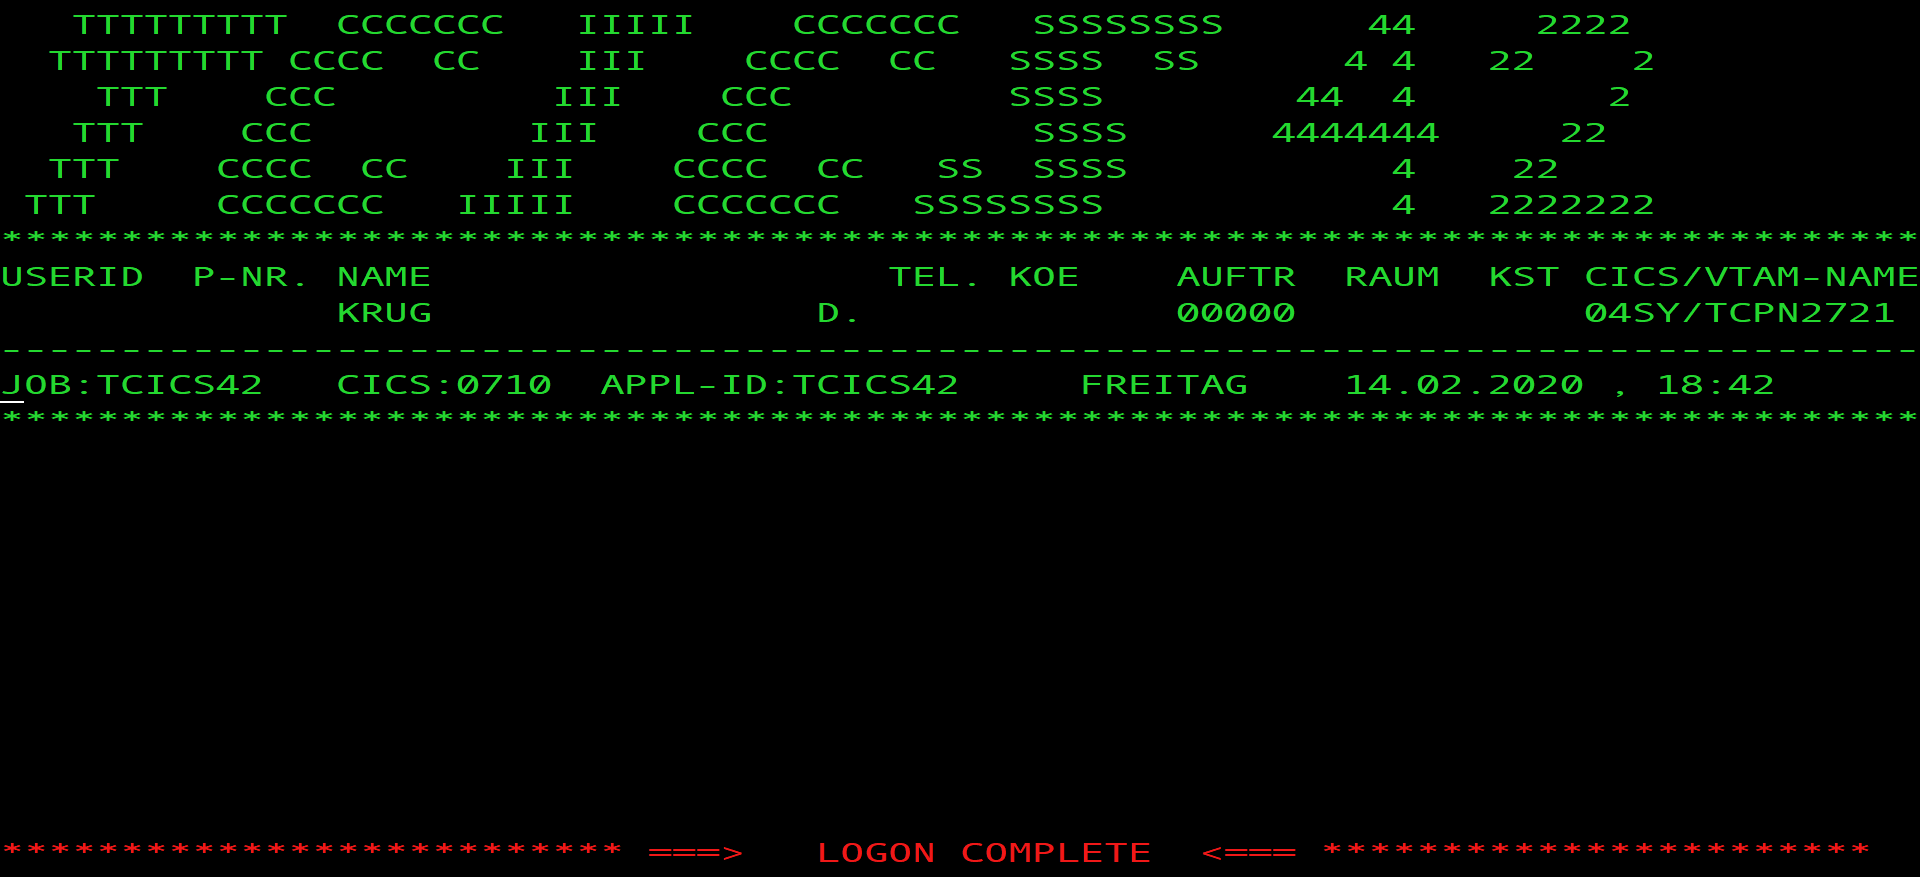
\includegraphics[width=\textwidth]{figures/logonscreen.PNG}
	\caption{Login Bildschirm der provisionierten DATEV spezifischen CICS-Instanz}
	\label{fig:cicslogin}
\end{figure}

\subsubsection{Bereitstellung Db2}\label{sssec:db2tpl}
In diesem Absatz wird die Provisionierung einer Db2 Datenbank beschrieben.
In der Systemumgebung Testplex bedeutet dies die Provisionierung der Datenbank ohne Tabelle und Daten.

Für die Erstellung einer Db2 Datenbank existiert innerhalb der DATEV e.G. eine REST-API.
Wie im Absatz \ref{sssec:workflow} beschrieben, ist es möglich, innerhalb eines Workflow Steps einen REST-Request abzusenden.
Der Code ist in Abbildung \ref{app:db2prov} im Anhang zu finden.
So muss im Body des Requests unter anderem der Datenbankname und eine UserID übergeben werden.
Der Code für das Löschen der Datenbank sieht ähnlich aus, nur handelt es sich in diesem Fall um einen DELETE-Request.
Die zwei notwendigen Steps wurden erzeugt und in den Workflow eingebunden.

Die API ist nur dazu fähig, Datenbanken auf einem bestimmten Datenbanksystem zu erzeugen.
Um die Datenbank aus der CICS-Instanz heraus nutzen zu können, muss dem CICS dieses Datenbanksystem mitgeteilt werden.
Hierfür ist, wie in Abbildung \ref{code:addCSD} in Zeile acht bereits zu sehen ist, das Hinzufügen einer weiteren CSD Gruppe notwendig ist, sowie die Aufnahme weitere Bibliotheken in der \glqq createCICS.jcl\grqq.
Dieser Aufruf wurde mittels neuer Variablen im Template möglichst dynamisch gestaltet und mussten in der Variableinputfile gesetzt werden.

\subsubsection{Bereitstellung IBM MQ}\label{sssec:mqtplx}
In diesem Absatz wird die Provisionierung einer IBM MQ Queue im Testplex beschrieben. 
Es ist auch möglich einen IBM MQ Queue Manager zu provisionieren, der Fokus dieser Arbeit liegt aber auf der Bereitstellung von Queues. 
Für die Bereitstellung eines IBM MQ Queue Mangers bei DATEV e.G. ist laut IBM MQ-Administration vorerst keine automatische Bereitstellung vorgesehen, gegebenenfalls kann dies in einem zukünftigen Szenario umgesetzt werden.
Ebenfalls in Abstimmung mit MQ- und CICS-Administration wurde entschieden, die Funktion eines Starts einer CICS Transaktionen über eine Queue vorerst nicht umzusetzen. Der Fokus lag auf der Prüfung, wie es möglich ist, eine einzelne Queue zu provisionieren, nicht die voll umfängliche Umsetzung der Anforderung der Anwendung DATEV-Rechnungsschreibung. 

Die IBM stellt Programme für die Verwaltung und das Nutzen von Queues  zur Verfügung.
Diese können mittels eines Jobs und bestimmten Parametern gestartet werden.
In Abbildung \ref{code:defq} ist die JCL des Jobs für das Erstellen einer Queue zu sehen.
Das auszuführende Programm ist \glqq CSQUTIL\grqq{} und als Parameter wird der Queuemanager übergeben.
Unter dem DD Namen \glqq MQSCIN\grqq{} ist der IBM MQ Befehl für das Erzeugen einer Queue zu sehen.
Um zu Prüfen, ob die Queue auch funktionsfähig ist, wurde nach dem Erstellen auch mit Hilfe eines Jobs, eine Message auf die Queue geschrieben und wieder abgeholt.
Der Job für das Löschen der Queues ist analog aufgebaut.

\begin{figure}[h]
	\centering
	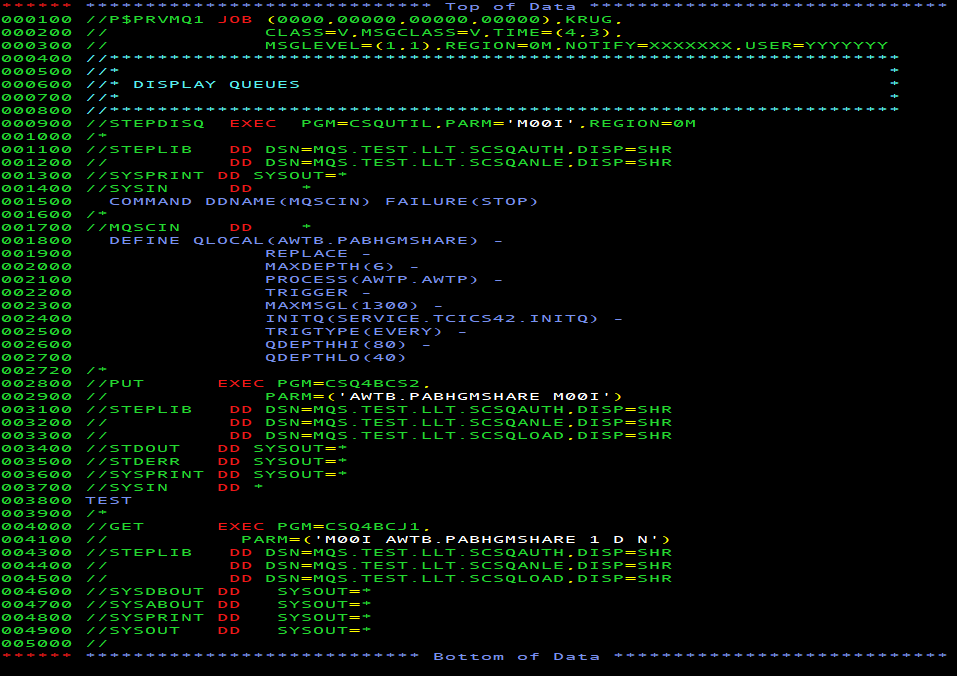
\includegraphics[width=\textwidth]{figures/defqjcl.PNG}
	\caption{Define IBM Queue, am Beispiel einer Trigger Queue}
	\label{code:defq}
\end{figure}

Ähnlich wie in Absatz \ref{sssec:db2tpl} für die Datenbank-Provisionierung beschrieben, muss der CSD Datei eine weitere Gruppe für den Queuemanager angegeben werden.
Zu sehen in Abbildung \ref{code:addCSD} in Zeile 11.
Dadurch hat die CICS-Instanz Zugriff auf alle Queues, die sich innerhalb dieses Managers befinden.
Des Weiteren ist die Aufnahme weiterer Bibliotheken in der \glqq createCICS.jcl\grqq{} notwendig.

\section{Entwicklungsstage}
Innerhalb der Entwicklungsstage sind die Sicherheits- und Rechtevorschriften schärfer als auf dem Test-Plex.
So wäre es zwar möglich, alle für die administrativen Aufgaben notwendigen Rechte einer persönlichen UserID zu geben.
Dies würde bedeuten, dass alle Anwender dieses Templates diese Rechte auch benötigen.
Damit bestünde eine potentielle Gefahr für das System, da sie damit auch außerhalb des Templates diese Rechte besitzen würden.
Somit wurde in Absprache mit den Administratorenteams für CICS und IBM MQ festgelegt, hierfür jeweils einen technischen User\footnote{User ID mit zunächst keinen Berechtigungen} zu beantragen.
Diesem werden nur die für das Template benötigten Rechte übergeben und er ist somit use-case-spezifisch.
Um als Anwender das Template nutzen zu können, werden nur die Rechte benötigt, Jobs mit diesen technischen Usern ausführen zu dürfen.
Für Db2 ist ein solcher User nicht notwendig, da das Datenbanksystem hinter der REST-API für alle zugänglich ist und jeder darauf Datenbanken erstellen darf.

Bei der Übertragung des Templates vom Test-Plex in die Entwicklungsstage waren Anpassungen in allen drei Bereichen des Templates notwendig.

\subsection{CICS Anpassung}
Dass der CICS spezifische technische User zum Einsatz kommt, musste der \glqq Job\grqq{} Baustein jeder JCL in jedem Step modifiziert werden.
Dafür bietet z/OSMF die Möglichkeit beim Zuweisen des \glqq Tenants\grqq{} eine Standard Jobkarte, die vor jeden Job des Templates eingefügt wird, zu hinterlegen.
Die CICS spezifischen Dateien können von der täglichen Datensicherung der Entwicklungsstage ausgeschlossen werden.
Da diese bei der Deprovisionierung gelöscht werden.
Um dies zu gewährleisten musste der Messageclass Parameter mit dem Wert  \glqq NONE\grqq{} angegeben werden.

Außerdem wird die CSD Datei, die als Vorlage gilt, durch die Standard Entwicklungsstage CSD Datei ersetzt.
In der Entwicklungsstage kommen im Vergleich zum Testplex andere Db2 und IBM MQ Bibliotheken zum Einsatz.
Dahingehend wurde die \glqq createCICS.jcl\grqq-Datei angepasst.
Zusätzlich musste ein SIT Parameter angepasst werden, so dass die Log Dateien funktionisfähig sind.
Eine weitere CSD Gruppe musste hinzugefügt werden.
Siehe Zeile 16 im Codeabschnitt \ref{code:createGrp}.
Diese sorgt dafür, dass die Bibliotheken, die die kompilierten Programme der kompletten Entwicklungsstage beinhalten, zur Verfügung stehen.
Außerdem kam noch eine neue Bibliothek hinzu.
Diese dient später als Ablageort der kompilierten Programme, die explizit nur in diese CICS-Instanz vorhanden sind.
Dies ist ein Standardvorgehen innerhalb der DATEV e.G. um neue Programmversionen zu testen.

\subsection{Db2 Anpassung}\label{ssec:db2entw}
Eine genauere technische Analyse der DATEV-Rechnungsschreibungsdatenbank kam zu dem  Ergebnis, dass es zwar möglich wäre diese Datenbank zu provisionieren, dies aber den zeitlichen Rahmen dieser Arbeit übersteigen würde.
Der Grund hierfür ist die Komplexität der benötigten Tabellen.
So wird auf drei Tabellen für die Ermittlung der Produktstammdaten lesend zugegriffen, auf neun weitere bei der Bestimmung der Preisabhängigkeiten.
Auf die Tabellen wird nicht direkt zugegriffen, sondern über Views\footnote{Alias eines Datenbankabfrage, auf die wie auf eine normale Tabelle zugegriffen werden kann}.
Bei den meisten werden innerhalb der View noch weitere Tabellen, teilweise aus anderen Datenbanken, gejoint.
Insgesamt besteht das System aus 14 Tabellen, die auf vier Datenbanken aufgeteilt sind, und 12 Views für den Zugriff auf diese Tabellen.

Die Db2 Administration muss dafür Vorarbeit leisten.
Mit dieser wurde begonnen, jedoch stellte sich heraus, dass die Komplexität (circa 600 Zeilen Code\footnote{Data Definition Language im Anhang \ref{app:ddl} zufinden} für einen kleinen Teil an Tabellen) der Anwendung DATEV Rechnungsschreibung im Rahmen dieser Arbeit als zu umfangreich angesehen wurde.
Sollte sich die Provisionierung generell als zielführend erweisen wird dieser Einmalaufwand erbracht werden.

Für die weitere Arbeit werden Datenbanken, die in einem anderen Datenbanksystem bereits vorhanden sind, genutzt.
Hierfür mussten die dafür vorgesehenen Variablen in der Eingabedatei des Templates angepasst werden.
Dadurch ändert sich die Gruppe in Zeile acht im Codeabschnitt \ref{code:addCSD} von \glqq DB0C \grqq{} auf \glqq DB0T \grqq.
Außerdem wurden sowohl in der Provisionierungs- als auch in der Deprovisionierungsdatei die Datenbanksteps auskommentiert und somit kommen diese nicht mehr zum Einsatz.

\subsection{IBM MQ Anpassung}\label{ssec:mqentw}
Da für die DATEV Rechnungsschreibung, wie im Absatz \ref{ssec:recharch} beschrieben, sehr viele gleichartige Queues benötigt werden, wurde für die Erstellung dieser von den IBM MQ Administratorenteam ein REXX Skript angefertigt.
Dies geschah unabhängig dieser Arbeit zum Zeitpunkt der Einführung des aktuellen DATEV Rechnungsschreibungsprozesses.
Dieses Skript steht dieser Arbeit zur Verfügung.
Für die Provisionierung IBM MQ Queues waren folgende Arbeitsschritte notwendig.

\begin{samepage}
\begin{itemize}
\item Anpassung des zur Verfügung stehenden Skriptes
\item Implementierung von Jobs für restliche Queues
\item Anpassung der CICS CSD Datei
\end{itemize}
\end{samepage}

Hierfür wurden zunächst die Eingabeparameter durch vorher angelegte Templatevariablen ersetzt.
Diese steuern, wie viele Queues jeweils angelegt werden, auf welchen Queue Manager die Queues angelegt werden und den ersten Qualifier des Queuenamens.
Für den restlichen Queuenamen existiert auch eine Variable, in dieser werden die Namen als Komma separierte Liste angeben und ausgelesen.
Anhand dieser Namen wird dann die maximale Queuetiefe und die maximale Länge einer einzelnen Nachricht festgelegt.
Im alten Skript wurden die Queues mit Hilfe einer Queue, die als Vorlage dient, angelegt.
Im Fall einer Provisionierung kann nicht davon ausgegangen werden, dass diese Vorlagen zur Verfügung stehen.
Deshalb wurden die benötigten Parameter explizit manuell angegeben.
Um die damit erstellten Queues zu testen, wurde eine Routine entwicklelt, die eine Nachricht auf die Queue schreibt und diese wieder abholt.
Anschließend wurde das Skript in den Provisionierungsworkflow mit Hilfe eines neuen Steps aufgenommen.

Für die Deprovisionierung der Queues besteht noch kein Skript.
Als Grundlage kann das vorher angepasste Provisionierungsskript dienen.
Hierfür musste der \glqq Define\grqq-Befehl für die Erstellung von Queues durch den \glqq Delete\grqq-Befehl ausgetauscht werden.
Die Logik für die Ermittlung der maximalen Queuetiefe und der maximalen Nachrichtenlänge wird dafür nicht mehr benötigt und konnte entfernt werden.

Die durch die beiden Skripte erstellten Queues sind nur für den Datenaustausch zwischen der CICS Transaktion für die Preisermittlung und dem Batch Ablauf zuständig.
Wie in Absatz \ref{ssec:recharch} beschrieben, benötigt der Ablauf noch weitere Queues.
Da es sich hierbei um spezielle Queues handelt, wurde auf die im Absatz \ref{sssec:mqtplx} gezeigte Technik zurückgegriffen.
Bei der Antwort-Queue für die Ermittlung der Listenpreise handelt es sich um eine Queue ohne besondere Parameter.
Es werden noch zwei Trigger-Queues benötigt, die über Prozesse eine Transaktion im CICS starten.
Als letzter Baustein für das Triggering der Transaktion wird noch eine Initiation Queue benötigt.
Diese muss im CICS hinterlegt sein.

Jeder CICS-Instanz kann nur eine Initiation Queue zugewiesen sein.
Dadurch benötigt jedes CICS eine eigene Initiation Queue.
Die Zuweisung geschieht in der IBM MQ CSD Gruppe.
Somit müsste für jede provisionierte CICS-Instanz im Voraus eine solche CSD Gruppe angelegt werden.
In Absprache mit der IBM MQ-Administrations  wurde entschieden, die Verwaltung der IBM MQ CSD Gruppe komplett dem Template zu übergeben.
Diese Entscheidung hatte eine Änderung des in Abbildung \ref{code:addCSD} gezeigten Codes zur Folge.
So wird, wie in Abbildung \ref{code:createGrp} dargestellt, zunächst eine Gruppe angelegt und erst anschließend dem CSD hinzugefügt.

\begin{minipage}{\linewidth}
\lstinputlisting[caption={Erstellung einer neuen CSD Gruppe},captionpos=b,label={code:createGrp}]{listings/InitAdditionalCSD.jcl}
\end{minipage}

Für jeden IBM MQ bezogenen Job wurde zuallerletzt die Jobkarte angepasst und der technische User der CICS-Administration durch den technischen User der IBM MQ-Admninistration, der für administrative Aufgaben berechtigt ist, ausgetauscht.

\subsection{Testablauf}
Für die Prüfung der Funktionsfähigkeit der so generierten Laufzeitumgebung steht dieser Arbeit ein Testablauf zur Verfügung.
Dieser wurde von den Mitarbeitern der DATEV Rechnungsschreibung beigesteuert.
Dabei handelt es sich um einen Teilablauf des gesamten DATEV Rechnungsschreibungsprozesses.
In diesem Ablauf wird nur die Preisermittlung, die die Laufzeitumgebung CICS benötigt, getestet.
Als Eingabe dienen vordefinierte Dateien und die Ergebnisse werden ebenfalls in Dateien geschrieben.
Der Ablauf liegt in Form von zwei Jobs vor.
Beide sind in der gleichen JCL Datei definiert, somit starten beide zeitgleich.
Dies ist notwendig, da der erste Job die Verarbeitung im CICS über die Queues startet und der zweite auf die Ergebnisqueues lauscht.

Um den Ablauf auch auf der vorher provisionierten Laufzeitumgebung zu starten, musste lediglich der verwendete Queue Manager angepasst werden.
Über die Queues und das verwendete Triggering wird die Transaktion im richtigen CICS gestartet.
Um die Ausgabe zu prüfen wurde der gleiche Testablauf mit den gleichen Eingabedateien auf der für Testzwecke üblichen Laufzeitumgebung durchgeführt.
Anschließend wurden die Ausgabedateien beider Läufe verglichen.

\section{Bereitstellungsprozess aktuelles Template}\label{sec:akttemp}
Bei dem Bereistellungsprozess, der durch das aktuelle Template möglich gemacht wird, sind drei Fälle zu unterscheiden:

\begin{samepage}
\begin{enumerate}
\item Fall:\\
Dem Entwicklerteam steht das Template in z/OSMF zur Verfügung und es wurde noch keine Instanz dieses Templates provisioniert.
Es wird eine neue Instanz benötigt.
\item Fall:\\
Dem Entwicklerteam steht das Template in z/OSMF zur Verfügung und es steht bereits eine Instanz dieses Templates zur Verfügung.
Es wird eine weitere Instanz benötigt.
\item Fall:\\
Das Administratorenteam führt Änderungen an einer Workflow Definitionsdatei durch.
Hier ist zwischen zwei weiteren Fällen zu unterscheiden:
\begin{enumerate}
\item Das Template wurde noch nicht veröffentlicht.
\item Das Template wurde veröffentlicht.
\end{enumerate}
\end{enumerate}
\end{samepage}

\subsection{1. Fall}
Der Mitarbeiter meldet sich an der zOSMF Oberfläche an und klickt auf den Menüleistenpunkt \glqq Cloud Provisioning\grqq.
Anschließend öffnet er die \glqq Software Services\grqq{} und wählt dort das oben genannte Template aus.
Er kann es ohne Änderungen provisionieren und damit seine Programmabläufe testen.

\subsection{2. Fall}\label{ssec:akttemp2fall}
Mit dem aktuellen Stand muss der Mitarbeiter wissen, an welchem Speicherort das Template abgelegt ist, da er die Template - nicht die Workflowdateien - kopieren muss.
Es sind Änderungen der Variableinputfile notwendig.
Unter anderem ist eine andere CICS Application ID zu wählen.
Um die Queues und IBM MQ Prozesse aus Fall eins nicht zu überschreiben, muss  ein anderer Queue Manager gesetzt werden.
Dieser Queue Manager muss von den zuständigen Administratorenteam manuell bereitgestellt werden.
Die Erzeugung einer von Fall eins unabhängigen Instanz setzt die Aufnahme eines neuen Templates, welches die veränderten Dateien beinhalten, in z/OSMF voraus.

\subsection{3. Fall}
Ein Template ist dann veröffentlicht, wenn es den berechtigten Teams zur Verfügung steht.
Zunächst muss der Speicherort der zu bearbeiteten Dateien bekannt sein.
Anschließend kann die Änderung mit einem Editor nach Wahl durchgeführt werden.

\subsubsection{3. Fall a)}
Hier kann das Template in der z/OSMF Oberfläche per Mausklick aktualisiert werden.

\subsubsection{3. Fall b)}
Um die Funktionsfähigkeit der veralteten Instanzen weiterhin sicherzustellen, muss eine neue Version des Templates erzeugt werden.
Dies ist auch per Mausklick zu lösen.

\section{Fazit Realisierung}
Am Ende der Realisierung steht ein funktionsfähiges Template.
Dieses Template provisioniert ein CICS und die benötigten IBM MQ Queues.
Wie in Absatz \ref{ssec:db2entw} beschrieben, wurde eine Db2 Datenbank wegen hoher Komplexität außen vorgelassen.
Auf dem Testplex wurde bewiesen, dass die Provisionierung einer Datenbank möglich ist.
Des Weiteren wäre die Provisionierung von Tabellen mit hohem einmaligen Arbeitsaufwand ebenfalls möglich.
Ein Testablauf der Beispielanwendung DATEV Rechnungsschreibung in einer provisionierten, isolierten CICS-Laufzeitumgebung konnte korrekt durchgeführt werden.

Folgende Probleme wurden im Rahmen der Implementierung erkannt:

\begin{samepage}
\begin{itemize}
\item Nicht sprechende Fehlermeldungen von z/OSMF
\item Nicht identifizierbare Programmiersprache
\item Nicht optimales Zugriffsrechtekonzept
\end{itemize}
\end{samepage}

Als erstes Problem sind nicht sprechenden Fehlermeldungen von z/OSMF, Abbildung \ref{fig:zosmffehler}, zu nennen.
\begin{figure}[h]
	\centering
	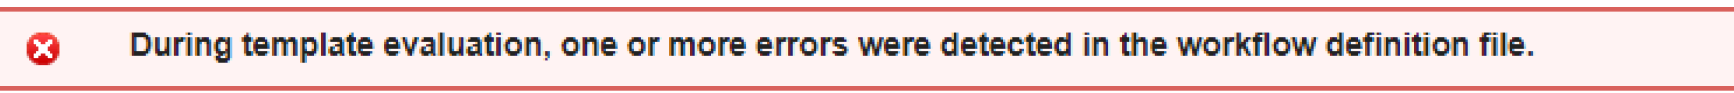
\includegraphics[width=\textwidth]{figures/zosmffehlermeldung.png}
	\caption{Beispiel einer Fehlermeldung von zOSMF}
	\label{fig:zosmffehler}
\end{figure}
z.B. wird bei dem Hinzufügen und Aktualisieren eines Templates in z/OSMF das Template und damit alle davon benötigten Dateien auf Syntaxfehler geprüft.
Die in Abbildung \ref{fig:zosmffehler} gezeigte Meldung tritt dann ein, wenn ein solcher Syntaxfehler vorhanden ist.
Es ist aber nicht zu erkennen, welcher Fehler genau vorliegt, noch nicht einmal in welcher Datei dieser auftritt.
Zudem auch keine genaue Anzahl an auftretenden Fehlern.
Dieser Umstand, kombiniert mit 36 bestehenden Dateien, erschwert die Fehlersuche.
Im Gegensatz dazu wird im Fehlerfall beim Ausführen eines Steps immer der Fehlercode und der genaue Ort des Fehlers ausgegeben.
Beispielsweise wird bei einem Step, in dem ein REST Aufruf durchgeführt wird, und ein Fehler auftritt, der Requestcode und die hinterlegte Fehlermeldung an der z/OSMF Oberfläche angezeigt. 

Ein weiteres Problem ist eine nicht genau identifizierbare Programmiersprache, die für die dynamische Generierung von Skripten genutzt wird.
So ermöglicht diese die dynamische Wertzuweisung von zum Beispiel REXX-Variablen durch Variablen des Templates.
Außerdem besteht eine Art von String Verarbeitung.
Zu beachten ist, dass wenn am Zeilenanfang ein \glqq\#\grqq{} steht, kann diese Programmiersprache verwendet werden.
In Abbildung \ref{code:qsauslesen} ist ein Beispiel zu sehen.
Dort werden die Queuenamen, die als kommaseparierte Liste in der Templatevariable \glqq DFH\_MQ\_QUEUENAMES\grqq{} angegeben sind, ausgelesen und in eigenen REXX Variablen gespeichert.
Zu sehen ist zunächst eine \glqq set\grqq{} Anweisung, mit der Variablen zugewiesen werden können, If-Bedingungen und eine foreach-Schleife stehen außerdem zur Verfügung.

\begin{minipage}{\linewidth}
\lstinputlisting[caption={Auslesen der \glqq DFH\_MQ\_QUEUENAMES\grqq{} Variablen und schreiben in REXX Variablen},captionpos=b,label={code:qsauslesen}]{listings/qsauslesen.rexx}
\end{minipage}

In Abbildung \ref{code:qsauslesenlaufzeit} wird das Ergebnis, welches zur Laufzeit ausgeführt wird, dargestellt.
Es ist zu erkennen, dass nur noch die für das REXX Skript notwendigen Codeabschnitte vorhanden sind.
Dadurch können sehr dynamische Templates erstellt werden.
Jedoch wurde weder eine Dokumentation zu dieser Sprache, noch um welche Sprache es sich genau handelt gefunden.
Somit liegt dem Wissen über diese Sprache nur der Code aus Beispielen der IBM zu Grunde.

\begin{minipage}{\linewidth}
\lstinputlisting[language=Rexx,caption={Zur Laufzeit erzeugtes Skript, der Grundlage aus Codeabschnitt \ref{code:qsauslesen}},captionpos=b,label={code:qsauslesenlaufzeit}]{listings/qsauslesenlaufzeit.rexx}
\end{minipage}

Ein weiterer Problempunkt ist das mit z/OSMF und dem Template einhergehende Zugriffsrechtekonzept.
Die z/OSMF Berechtigungsgruppen sind nicht an die DATEV e.G. internen Richtlinien angepasst.
Die Aufnahme in eine solche Gruppe, um zum Beispiel die z/OSMF Oberfläche nutzen zu dürfen, geschieht auf Zuruf und manuelles Hinzufügen einer User ID durch einen Mitarbeiter.
Außerdem ist der Einsatz einer für das ganze Template gültigen Standard Jobkarte, um technische User verwenden zu können, nicht optimal.
z/OSMF bietet hier eigentlich eine Möglichkeit in der Stepdefinition einen \glqq runAsUser\grqq{} anzugeben.
Unter diesem User würde der Step dann ausgeführt werden.
Folglich ist das die Stelle an der zum Beispiel für CICS Steps der technische User für administrative CICS Aufgaben angegeben werden müsste.
So würde das Gewähren der expliziten Rechte zum Starten eines Jobs mit der technischen User Id entfallen und damit die manuelle Arbeit des \glqq Gewährens\grqq, was mittels eines Formulars beantragt wird.
Jedoch um einen \glqq runAsUser\grqq{} in der Stepdefinition angeben zu können, muss in der dem Template zugewiesen \glqq Domain\grqq{} ein sogenannter \glqq Cloud Security Admin\grqq{} hinterlegt sein.
Dieser würde sicherstellen, dass nur die für ein Template zugelassenen User dieses Template auch provisionieren dürfen.
In dieser Arbeit wird die mitgelieferte \glqq Default Domain\grqq{} genutzt, in dieser ist kein \glqq Cloud Security Admin\grqq{} angegeben.
Da es sich um die Standard \glqq Domain\grqq{} handelt, darf diese nicht geändert werden.
Somit müsste eine eigene \glqq Domain\grqq{} angelegt werden um einen \glqq Cloud Security Admin\grqq{} hinterlegen zu können.
Dadurch, dass sich z/OSMF bei der DATEV e.G. noch in einem Teststadium befindet, wird von der Erstellung einer eigenen \glqq Domain\grqq{} abgesehen.
Dies ist der Grund für den nicht optimalen Einsatz der oben genannten Jobkarten.
An diesen beiden Fällen ist zu erkennen, dass das Rechtekonzept noch nicht für einen firmenweiten Einsatz ausgelegt ist und noch überarbeitet und angepasst werden muss.
Dies ist jedoch explizit nicht Bestandteil dieser Arbeit.


 

\section{Interviews}
In diesem Absatz wird zunächst erläutert, auf welcher Grundlage (Kommentar: was heißt hier Grundlage?) die Interviews geführt wurden.
Anschließend werden die Ergebnisse der einzelnen Interviews nach Gruppen aufgeteilt, ausgewertet und interpretiert.
Schließlich wird daraus ein allgemeines Stimmungsbild abgeleitet.

\subsection{Durchführung}
Interviewt wurden jeweils zwei Mitarbeiter der Gruppen, CICS Administration, Db2 Administration, IBM MQ Administration.
Zusätzlich wurde eine Fachberaterin im Bereich Technologiestrategie und ein Mitarbeiter (Kommentar: wirklich nur einer?) des Entwicklerteams der DATEV Rechnungsschreibung befragt.
Für die beiden letztgenannten Interviews waren nur die Fragen 1., 2. und 6. bis 10. des Fragebogens von Relevanz.
Sowohl der Fragenkatalog, als auch die ausgefüllten und digitalisierten Fragebögen sind im Anhang \ref{app:fragen} zu finden.
Vor Durchführung der Interviews, wurde den Teams in getrennten Terminen die Ergebnisse dieser Arbeit vorgestellt.
Der Schwerpunkt der Vorstellung wurde an das jeweilige Team angepasst.
So wurde bei den Administratorenteams vor allem auf die Erstellung der Templates, was für ihr Arbeitsgebiet relevant ist, eingegangen.
Außerdem wurde neben der im Absatz \ref{sec:akttemp} dargestellten Lösung (Kommentar: welche?), auch die Lösung aus Kapitel \ref{ch:ausblick} (Kommentar: welche?) vorgestellt.
An Hand des durch diese Arbeit bereit gestellten Templates wurde die z/OSMF Oberfläche erläutert.

\subsubsection{CICS Administratoren}
Die Einschätzung des Werts des aktuell möglichen Ablaufs mittels z/OSMF von CICS Administrator 1 ist mittelmäßig.
So bietet es zwar eine flexible Versionierung und Veröffentlichung, jedoch ist es durch die verschiedenen Sprachen und Dokumentarten (Kommentar: siehe ....  einfügen)  mit Startschwierigkeiten versehen. (Kommentar: vlt. eher etwas spezifischer, EInarbeitungsaufwand??)
Im Gegensatz dazu sieht CICS Administrator 2 das momentane Template zumindest für CICS als ablauffähig und mehrfach einsetzbar. (Kommentar: das ist kein Gegensatz zu Admin1, vlt. eher: Dagegen bewertet CICS Admin 2 das Template...... )
Beide Administratoren sehen einen Vorteil in der z/OSPT Lösung, d.h. der Konfigurierbarkeit  außerhalb des Templates 
Als Nachteil bewerten sie jedoch die Notwendigkeit eines sehr dynamischen Templates (KOmmentar: der Nachteil ist nicht die Notwendigkeit, sondern, dass das Template durch die notwendige Komplexität sehr komplex wird.
Die Benutzerfreundlichkeit der Oberfläche wird von CICS Administrator 1 für beide Lösungen (z/OSMF Und z/OSPT) mit sehr gut bewertet.
Auf Grund dessen, dass er noch nicht damit gearbeitet hat, enthält sich CICS Administrator 2 hier der Bewertung.
Die Arbeitsweise bei Änderungen an den Workflow Definitionsdateien und dahinterliegenden Skripten usw., wird als schlecht bis mittelmäßig eingeschätzt.
Hier fehlt beiden Befragten eine geeignete Toolunterstützung, z.B. auch mit Syntaxhighlighting.
Der erste Eindruck wird von einem hohen Ersteinrichtungsaufwand und einer zeitaufwändigen Einarbeitungsphase geprägt.
Zusammen mit den verschiedenen Sprachen hat dies auf CICS Administrator 1 eine eher abschreckende Wirkung.
Dennoch können sich beide Befragten vorstellen, nachdem der Einarbeitungsaufwand erbracht wurde, täglich mit dem Toolkit zu arbeiten, da bei dem aktuell etablierten Prozess ein hoher manueller Aufwand zu erbringen ist und eine Abstimmung zwischen den Administratoren und dem Entwicklerteam notwendig ist.

Zusammenfassend lässt sich sagen, dass die CICS Administratoren eine Chance auf Verbesserung des Prozesses durch das Toolkit sehen.
Allerdings schreckt der hohe Einarbeitungsaufwand und die Mischung aus verschiedenen Sprachen und fehlendem Syntaxhighlighting bei der Templateerstellung ab.

\subsubsection{Db2 Administratoren}
Sowohl Db2 Administrator 1 als auch Db2 Administrator 2 erkennen die Möglichkeit einer Verbesserung durch z/OSMF.
Jedoch sind sie der Meinung, dass noch einiges an Forschung und Weiterentwicklung notwendig ist um es sinnvoll nutzen zu können.
Sie stimmen auch bei ihrer Ansicht bezüglich z/OSPT überein.
So sehen sie den Vorteil des Kommandozeileninterfaces vor allem bei einer Endausbaustufe mit automatisiertem Deployment innerhalb einer CI/DC-Pipline und dem Einsatz von Jenkins basierten Builds und Tests.
Db2 Administrator 2 stört sich an den Begriffen \glqq Container\grqq{} und \glqq Image\grqq, da diese teilweise vertauscht und synonym verwendet werden. (Kommentar: von wem? Von Dir oder von IBM?)
Bezüglich der Benutzerfreundlichkeit der Oberfläche fällt die Bewertung bei beiden schlecht bis mittelmäßig aus.
Db2 Administrator 1 empfindet die gezeigte Arbeitsweise für Änderungen an den Workflow Definitionsdateien als sehr schlecht, da es momentan ohne automatisches Deployment realisiert ist.
Die Bewertung von Db2 Administrator 2 ist mittelmäßig, da eine Entwicklungsumgebung sinnvoll wäre, vor allem in Hinblick auf eine Syntaxprüfung.
Der erste Eindruck des Toolkits ist sehr positiv. (Kommentar: damit ist wieder z/OSPT gemeint, oder?)
Es wird als mächtiges Tool und als Zukunft des modernen Deployments auf dem Mainframe eingeschätzt, jedoch wird es als sehr komplex betrachtet.
Im Vergleich dazu wird der aktuell etablierte Bereitstellungsprozess ebenfalls als komplex beschrieben.
Dieser funktioniere zwar sehr gut, aber es sind viele Abhängigkeiten zu anderen Personen vorhanden, dadurch entstehen Wartezeiten.
Außerdem sei ein sehr umfangreiches Wissen über alle beteiligten Subsysteme notwendig.
Hinzu kommt ein hoher Konfigurationsaufwand und viel Vorarbeit, zum Beispiel Funktionsuser und ein Rechtekonzept.
Beide Db2 Administratoren könnten sich  vorstellen mit dem Toolkit täglich zu arbeiten, um diese Probleme anzugehen.
Eine INtegration mit einer Jenkins-basierten Build-Pipeline wird hierfür von Db2 Administrator 1 vorausgesetzt.

Die Interviews mit den Db2 Administratoren ergaben folgendes Bild.
Sie sehen in dem Toolkit eine gute Möglichkeit, um den Bereitstellungsprozess zu vereinfachen und weniger zeitaufwändig zu gestalten.
Allerdings ist noch viel Forschungsarbeit in dieses Thema zu investieren.
Als Hauptpunkt ist die Nutzung von Jenkins und damit die Einbindung und Etablierung einer automatisierten Build-Pipeline zu nennen.

\subsubsection{IBM MQ Administratoren}
IBM MQ Administrator 1 sieht bereits im aktuell funktionsfähigen Template einen Mehrwert.
Zum einen, weil mehr Verantwortung im Entwicklerteam liegt und zum anderen sind weniger manuelle Eingriffe bei der Bereitstellung durch die MQ-Administrtion notwendig.
Jedoch ist die Lösung, die im Ausblick gezeigt wurde (Kommentar welche? ...) , flexibler und damit etwas besser geeignet.
Zudem seien die momentan bereits vorhandenen Features (Kommentar: welche? Meinst du den momentan vorhandenen Prozess???) durchaus gut, jedoch kam die Frage auf, ob die IBM das `IBM Cloud Provisioning and Management for z/OS`-Toolkit noch weiterentwickeln wird.
Die Benutzerfreundlichkeit der z/OSMF Oberfläche wurde als mittelmäßig bis gut eingestuft.
Bezüglich des Arbeitens, Verwaltens und Änderns von Workflow Definitionsdateien und der dazugehörigen Skripte konnte keine Bewertung abgegeben werden, da noch nicht selbst damit gearbeitet wurde (Kommentar: DU hast es ihnen ja gezeigt, d.h. wenn dann müsstest du schreiben, wollten die Kollegen nur aufgrund der Demo und ohne selbst damit gearbeitet zu haben, keine Bewertung abgeben)
Dies hat auch Einfluss auf den ersten Eindruck. 
So wird zu bedenken gegeben, dass der Zeitaufwand und die zu leistenden Vorarbeiten mit einzubeziehen (Kommentar: in was? in d ie Bewertung? sind.
Vor allem, wenn die Provisionierung von einem IBM MQ Queue Manager hinzu kommt (Kommentar: wo hinzu, die aktuell noch Manuelle Bereitstellung oder die, die noch im Toolkit dazu kommt? Missverständlich).
Jedoch kann sich IBM MQ Administrator 1 vorstellen mit dem Toolkit täglich zu arbeiten, da letztendlich die Werkzeugwahl keine Rolle spielt. (Kommentar: welche Werkzeugauswahl? Bei was spielt sie keine Rolle?)
Diese Einschätzung  wird dadurch begünstigt, dass der aktuell etablierte Prozess schlecht beurteilt wird, aufgrund des hohen manuellen Aufwands und der dadurch erzeugten Rückfragen mit den Beteiligten.
Zuletzt wird noch darauf hingewiesen, dass das Toolkit generell noch Neuland sei.
So müssten erst die Grundlagen gelernt und damit Erfahrungen gesammelt werden bevor eine qualifizierte Bewertung möglich sei. (Kommentar: das kommt nicht so gut rüber, so als ob du es ihnen noch nicht gut genug gezeigt hättest. Vlt. eher die  "endgültige qualifizierte Bewertung)

Im Vergleich zu IBM MQ Administrator 1 fehlen IBM MQ Administrator 2 noch weitere Automatismen.
So sind trotz des Einsatzes von z/OSPT noch Absprachen mit Dritten, wie dem RACF-Team und dem Speicher-Team, notwendig.
z/OSPT sei zudem zwar "Docker ähnlich", ist jedoch keine vollumfängliche Containerlösung.
So könnte sich IBM MQ Administrator 2 zwar vorstellen, dass Entwickler dem Toolkit täglich  arbeiten, aber es müsste ohne manuelle Eingriffe funktionieren. (Kommentar: was heißt hier täglich arbeiten... das erstellen eines Toolkit-Templates kann nicht ohne manuelle Eingriffe funktionieren... Das ist ja der Job der Admins. Die manuellen Eingriffe werden für den Entwickler wegfallen, nicht für den Admin)
Die Erstellung der Skripte muss mit einem einmaligen Aufwand verbunden sein, so dass sie keine ständigen Anpassungen benötigen.
Davon wird auch der erste Eindruck beeinflusst.
Insgesamt sind seiner Meinung nach zwar viele gute Ansätze vorhanden, aber es fehlen Analogien und eine Ähnlichkeit zu Jenkins-Skripten, die mit groovy, yaml oder ansible playbooks arbeiten, XML "sei nicht mehr zeitgemäß". 

Zusammenfassend lässt sich sagen, dass sich beide IBM MQ Administratoren einig sind, dass der momentan etablierte Bereitstellungsprozess nicht mehr gut genug (Kommentar: passt das?) ist und ein neuer Prozess durchaus notwendig wäre.
Der durch diese Arbeit gezeigte Prozess als Ablöse wird als prinzipiell möglich erachtet, jedoch nur der Einsatz mit z/OSPT.
Außerdem wird vor einer hohen Lernkurve und der noch fehlenden Automation, sowie der fehlenden Ähnlichkeit zu Jenkins oder anderen PaaS Lösungen (Kommentar: nochmal: welche?) gewarnt.

\subsubsection{Entwicklerteam der DATEV Rechnungsschreibung}
Aus Sicht des Entwicklers wird für den gezeigten Bereitstellungsprozess viel Wissen über die z/OSMF Oberfläche und das Template selbst benötigt. (Kommentar: eigentlich muss er das ja nicht wissen. d.h. wenn er den Eindruck hat, dann wäre die Demo nicht gut gewesen...)
Dieses Wissen müsse auch bei nicht häufiger Nutzung über einen längeren Zeitraum erhalten werden.
Der Prozess sei zwar schon "ganz gut", jedoch sei weiterhin viel Absprache mit den Administratoren notwendig. (Kommentar: ist das so?)
Hier wird auch der Nachteil des momentan etablierten Bereitstellungsprozesses gesehen.
Jedoch sobald der Erstaufwand für die Einarbeitung in z/OSMF geleistet wurde, muss sich nur im Ausnahmefall noch darum gekümmert werden.
Diese Verantwortung würde im Fall der Umsetzung mit z/OSPT bei dem Entwicklerteam selbst liegen. (Kommentar: das ist echt schwierig zu verstehen, lass uns das morgen mal umformulieren auf Basis der Interview-Unterlagen).
Durch die eingesparten Absprachen erhofft man  sich eine höhere Effizienz im  (KOmmentar: in was? tägliche Arbeit? WEnn das so wäre dann widerspricht das der "nicht häufigen Nutzung oben).
Es wurde noch die Nutzung in der Qualitätssicherungs- und Produktionsstage genannt.
Hier werden Vorteile einer einfache Skalierbarkeit gesehen. (Kommentar: zu oberflächlich: versteht man nicht. für die Zukunft könnte man sich die Nutzung auch für die QS_ und Prod-Stage vorstellen, und dort z.B. auch CICS-Umgebungen horizontal skalieren. Dies ist jedoch nicht Teil der vorliegenden Arbeit).
Vor allem auf Grund der Eigenverantwortung über die Subsysteme (Kommentar: über das Management der eigenen Testssysteme mit den Subsystemen) könnte man sich die tägliche Arbeit mit dem Toolkit vorstellen.
Allerdings nur in Hinblick auf eine Integration in eine Jenkins Build Pipeline, für die erst einmal Sammeln von Erfahrungen bezüglich des Prozesses und des Toolings notwendig wären.

Das Hauptaugenmerk des Entwicklers liegt bei der höheren Eigenverantwortung beziehungsweise der Eigenverwaltung von benötigten Subsystemen.
Eine einfache und intuitive Bedienung des Toolkits ist außerdem wichtig.

\subsubsection{Fachberaterin im Bereich Technologiestrategie}
Laut der Fachberaterin im Bereich Technologiestrategie ist der gezeigte Ablauf beziehungsweise die z/OSMF Oberfläche für eine solche Aufgabe (Kommentar: für die Aufgabe des Provisionierens von z/OS Middleware) geeignet.
Jedoch sei es besser wenn z/OSMF in den bereits existierenden \glqq Marktplatz\grqq{} für DATEV Cloud Lösungen integriert wäre.
Der Prozess, der mit Hilfe von z/OSPT ermöglicht wird, wird als gut angesehen, da durch ihn die Entwicklung von z/OS Anwendungen an die Vorgehensweise der Cloud Native Entwicklung angenähert wird.
Hier kommt die Rolle des Build Engineers auch für solche Anwendungen ins Spiel.
Dieser kümmert sich um die Erstellung und Pflege der Build-Pipeline.
Große Nachteil im momentan etablierten Bereitstellungsprozess sei vor allem,  dass eine Anzahl vpn Entwicklern, die parallel an einem Produkt arbeiten, sich die gleiche Entwicklungssystemumgebung teilen.
So arbeiten alle mit der gleichen CICS-Instanz, der gleichen Test-Datenbank und mit den gleichen IBM MQ Queues.
Dadurch beeinflussen Änderungen des einen Entwicklers die Tests der anderen Kollegen, es entsteht Koordinationsaufwand.
Falls Änderungen an der Umgebung notwendig sind, kann während dieser Zeit kein Entwickler weiterarbeiten.
Hier liege der Vorteil des Toolkits.
Es ermöglicht aus Entwicklersicht eine sehr einfache, schnelle Möglichkeit eine isolierte Umgebung bereitzustellen, unabhängig von den Administratorenteams.
Zusätzlich dienen die Konfigurationsdateien auch als Dokumentation, welche Ressourcen für ein erneutes Erstellen der Umgebung notwendig sind.

Abschließend lässt sich sagen, dass aus Sicht einer Fachberaterin im Bereich Technologiestrategie dieses Toolkit die Entwicklung beziehungsweise den Bereitstellungsprozess deutlich verbessern kann.
So ist für den Entwickler ein an die Cloud Native Welt angenäherter Entwicklungsprozess möglich.
Dadurch wird der Wechsel zwischen beiden Umgebungen immer fließender.

\subsection{Meinungsbild}
Über alle Gruppen hinweg lassen sich folgende Punkte zusammenfassen:

\begin{samepage}
\begin{itemize}
\item neuer Prozess notwendig
\item z/OSPT Lösung bevorzugt
\item erste Erfahrungen sammlen
\end{itemize}
\end{samepage}

Es stimmen alle Gruppen überein, dass der momentan etablierte Bereitstellungsprozess für Mainframesubsysteme durch viele Absprachen und Abstimmungs-Aufwand zeitaufwändig ist.
Sie würden einen neuen, schnelleren Prozess begrüßen. (Kommentar: automatisiert!!)

Jedoch muss dieser Prozess aus Entwicklersicht mit minimalem Konfigurationsaufwand verbunden sein.
Dies könnte durch eine Provisionierung mittels z/OSPT und einer  Integration in eine Jenkins Build Pipeline oder durch die Einbindung in den \glqq DATEV Marktplatz\grqq{} mittels eines entwickelten \glqq Service Brokers\grqq. gewährleistet werden.
Aus Sicht der Administratoren sind mit dieser Umsetzung nur wenige allgemeine Templates zu verwalten, da die Entwickler mit z/OSPT Images und keine weiteren Templates erzeugen.
Um diese Punkte zu ermöglichen, muss das Template umgestaltet werden.
Der dadurch in den Administratorenteams entstehende Aufwand und die damit verbundene steile Lernkurve hat eine abschreckende Wirkung.

Trotz dieser abschreckenden Wirkung sind auch die Administratorenteams bereit, falls die Kapazitäten vorhanden sind, den Bereitstellungsprozess mit Hilfe des \glqq IBM Cloud Provisioning and Management for z/OS\grqq{} zu verbessern.
Aus Sicht der Technologiestrategie ist dies ein wichtiger und notwendiger Schritt hin zu einem Cloud Native ähnlichen Prozess.

\chapter{Ausblick}\label{ch:ausblick}
Je weiter sich das Projekt der vorliegenden Arbeit dem Abschluss näherte, desto mehr kristallisierte sich ein Hauptproblem für den praktischen Einsatz heraus.
Das erstellte Template ist sehr auf die DATEV-Rechnungsschreibung spezialisiert, das heißt es ist funktionsfähig, kann aber nicht ohne zeitaufwändige Eingriffe in das Template, in die Workflowdefinitionsdateien und die eigentlichen REXX Skripte und Jobs, an eine andere Anwendung angepasst werden. 
Folglich müsste das Template dynamischer implementiert sein.
Um dies zu verdeutlichen, wird als Beispiel die Provisionierung von IBM MQ Queues herangezogen.
Momentan werden die Prozesse und die Trigger Queues statisch angelegt.
Das heißt, dass sowohl Namen, als auch die damit verknüpften Queueparameter, fest hinterlegt sind, um nur ein Beispiel zu nennen.
Besser wäre es, alle Parameter in der Eingabedatei des Templates anzugeben.
Aus IBM MQ Sicht ist hinzuzufügen, dass die fehlende automatisierte Bereitstellung eines Queue Managers den gewünschten Effekt einer weitgehenden Automatisierung und Unabhängigkeit von der Administration, abschwächt.

Während der Realisierung stellte sich ebenfalls heraus, dass ein Template, das mehrere Subsysteme beinhaltet und dadurch sehr anwendungsspezifisch ist, nicht für einen firmenweiten Einsatz geeignet ist.
So ist zu empfehlen, dass für jedes Subsystem, also CICS, Db2 und IBM MQ, ein separates \glqq Basis\grqq-Template realisiert wird.

Angenommen es besteht für jedes Subsystem ein Template und das IBM MQ Template beinhaltet die Provisionierung eines Queue Managers, so könnte jeder Entwickler seine eigenen Instanzen der Templates besitzen und für eigene Tests nutzen.
Dennoch wäre der ermöglichte Bereitstellungsprozess nicht optimal.
So müsste für jede kleine Änderung an der Konfigurationsdatei ein neues Template erzeugt werden, siehe zweiter Use-Case im Abschnitt \ref{ssec:akttemp2fall}.
Das dort genannte Beispiel einer CICS-Instanz und der notwendigen eindeutigen Application ID wird hier aufgegriffen.
Eine Möglichkeit dieses Problem zu lösen, wäre einen Pool mit verfügbaren Application IDs bereitzustellen und dann mittels eines Programms eine ungenutzte Application ID zu ermitteln.
Dieses Programm könnte dann als Step in das Template aufgenommen werden.
Jedoch müsste immer noch für jede Änderung an der Konfigurationsdatei ein neues Template erzeugt werden.

Hier schafft z/OSPT Abhilfe.
Damit kann, wie in Absatz \ref{sssec:zospt} beschrieben, mit Hilfe der z/OSPT-Datei und dem Konzept der Images das Template von außen konfiguriert werden.
Dadurch fällt das Kopieren des Templates für den Mitarbeiter weg, dieser kann mittels des Kommandozeileninterfaces ein z/OSPT-Image bauen und daraus einen z/OSPT-Container erzeugen.
Das Kommandozeileninterface hat einen weiteren Vorteil.
Mit dessen Hilfe können Arbeitsschritte für die Provisionierung der Middleware über groovy in einen Jenkins-Ablauf aufgenommen werden.
Somit läuft der Prozess automatisiert ab und nähert sich modernen Entwicklungsabläufen wie denen aus der Cloud Native Entwicklung an.

Angenommen es existieren jeweils ein CICS, ein Db2 und ein IBM MQ Template, und diese sind so realisiert, dass sie firmenweit eingesetzt werden können.
Dann wäre der nächste Schritt, die Aufnahme in den \glqq DATEV Marktplatz\grqq, möglich.
Der \glqq DATEV Marktplatz\grqq{} ist eine Weboberfläche, mit der sich Entwicklerteams ihre benötigte PaaS-Umgebung konfigurieren können.
Heute stehen ihnen dort Dienste wie MongoDB, PostgreSQL, Kafka und viele weitere zur Verfügung.
In Zukunft könnten hier auch Dienste wie CICS, Db2 und IBM MQ zur Auswahl stehen.
Dabei ist in Betracht zu ziehen, ob für den User nur bestimmte vorgefertigte Profile, wie \glqq klein\grqq, \glqq mittel\grqq{} und \glqq groß\grqq, auswählbar sind. 
Dies ist in public Clouds bzw. auch bei der DATEV PaaS Lösung ein übliches Vorgehen.
Die im Hintergrund verbundenen Templates und Images müssten dahingehend angepasst werden.
Um einen solchen \glqq Service Broker\grqq{} zu verwirklichen, könnte die von z/OSMF zur Verfügung gestellte REST-API verwendet werden.
Diese ermöglicht den Zugriff auf fast alle z/OSMF Funktionalitäten mittels Http-Requests.
Für die Tenant Zuweisung zu einem Template würde weiterhin die z/OSMF Oberfläche benötigt werden.
Insgesamt ist zu erkennen, dass mit z/OSMF beziehungsweise IBM hier noch Verbesserungen machbar sind.

Diese technische Umsetzung ermöglicht in Zukunft den in Diagramm \ref{fig:proneu} dargestellten Bereitstellungsprozess.
Es ist zu erkennen, dass Verantwortung für die Bereitstellung einer Laufzeitumgebung in der Entwicklungsstage von den Administratorenteams an die Entwicklerteams übertragen wird.
Dadurch wird Kommunikationsaufwand eingespart und einem Entwickler steht binnen weniger Minuten eine funktionsfähige Laufzeitumgebung in der Entwicklungsstage für seine legacy z/OS Anwendung zur Verfügung.
Bei Problemen oder Beratungswunsch unterstützen die Administratorenteams weiterhin.
Der Hauptaufwand der Umsetzung dieser Lösung liegt bei den Administratorenteams.
Der Effizienzgewinn stellt sich ein, wenn für die wichtigsten Anwendungen Templates existieren, die von den Entwicklern jederzeit genutzt werden können, um in isolierten, individuellen Umgebungen zu entwickeln und zu testen.

\begin{figure}[ht!]
\centering
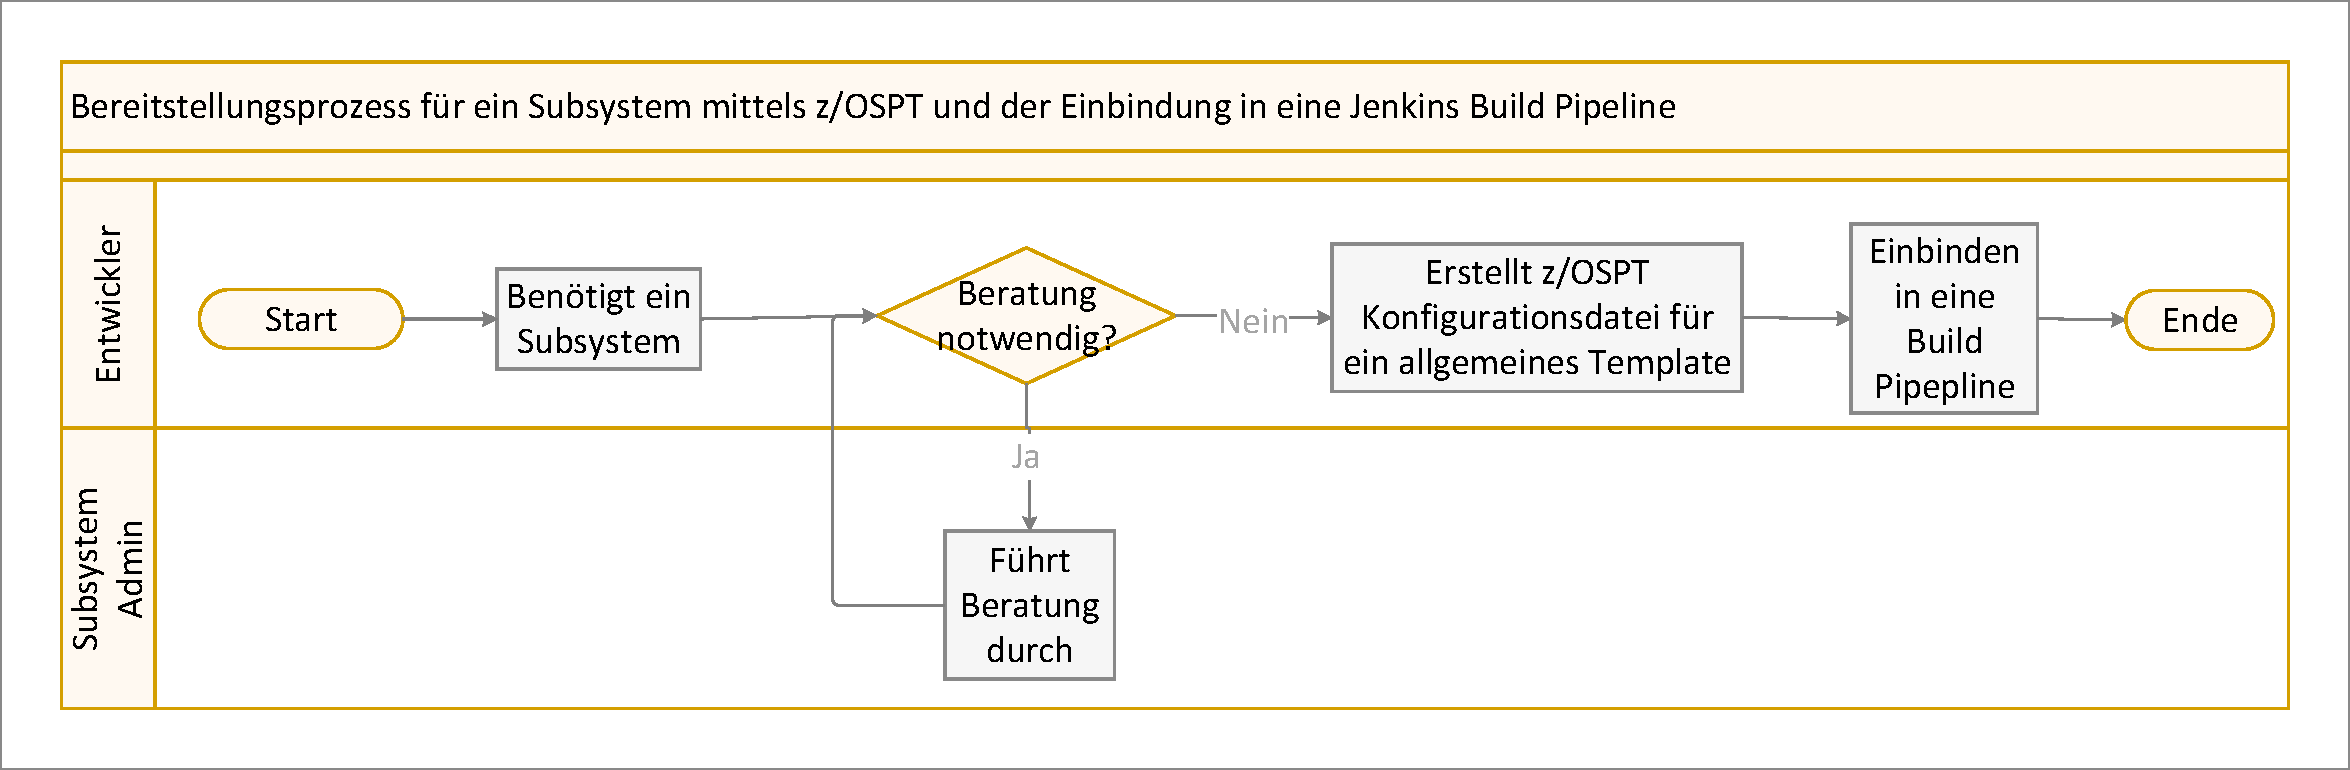
\includegraphics[width=\paperwidth,angle=90]{figures/swimlaneNeuerProzess.pdf}
\caption{Bereistellungsprozess eines Subsystems mittels einer z/OSPT Konfigurationsdatei}
\label{fig:proneu}
\end{figure}

Ist all dies umgesetzt, kann in einem nächsten Schritt der cloud native Aspekt des automatisierten Deployments einer Anwendung inklusive Laufzeitumgebung zwischen Stages bis hin zur Produktion auch für z/OS Anwendungen in Betracht gezogen werden.

\chapter{Zusammenfassung und Fazit}\label{ch:zusammenfassung}
Zusammenfassend lässt sich sagen, dass es generell möglich ist mit \glqq IBM Cloud Provisioning and Management for z/OS\grqq{} Laufzeitumgebungen für legacy z/OS Anwendungen automatisiert bereitzustellen.
Wie aus Tabelle \ref{tab:zosvscn} zu erkennen ist, ist es in einem gewissen Grad auch möglich damit den Bereitstellungsprozess für z/OS Anwendungen bei DATEV e.G. an den cloud native Prozess anzunähern.

\begin{table}[h]
\centering
\begin{tabularx}{\textwidth}{p{5cm}|X|X}
& \glqq IBM Cloud Provisioning and Management for z/OS\grqq & cloud native \\
\hline
Produkt-Teams & nein & ja \\
\hline
automatisierte Bereitstellung von Laufzeitumgebungen in der: &  &  \\
Entwicklungsstage & ja & ja\\
Qualitätssicherungsstage & nein & ja\\
Produktionsstage & nein & ja\\
\hline
CI/CD-Pipeline Unterstützung & ja, mit z/OSPT & ja \\
\end{tabularx}
\caption{Verlgeich von \glqq IBM Cloud Provisioning and Management for z/OS\grqq und cloud native im Bezug auf ihren Bereitstellungsprozess}
\label{tab:zosvscn}
\end{table}

Die Annäherung beschränkt sich jedoch nur auf eine automatisierte Provisionierung von Laufzeitumgebungen in der Entwicklungsstage.
Es werden noch keine Produkt-Teams gebildet, sondern auch mit den Einsatz von \glqq IBM Cloud Provisioning and Management for z/OS\grqq{} bleibt die Verwaltung und Überwachung der Middleware bei den Administratorenteams.

Wird der z/OSMF Lösungsansatz genauer betrachtet, dann ist zu erkennen, dass dieser durch den Abbau der Kommunikation zwischen den Abteilungen und nur einmaligem Erstellen der Skripte weniger fehleranfällig und effizienter als der momentan etablierte Prozess ist.
Jedoch ist es noch nicht perfekt.
Der Bereitstellungsprozess ist noch immer mit einigen manuellen Schritten verbunden.
So muss das Template manuell kopiert werden und Änderungen an der Konfiguration müssen innerhalb des Templates stattfinden.

Hierfür wurde in der Arbeit eine Lösung mit Hilfe von z/OSPT beleuchtet.
Diese sieht in einer Endausbaustufe eine einfache Einbindung des Templates in einen automatisierten Build-Prozess, zum Beispiel mit Jenkins, vor.
Außerdem würde der Einsatz von z/OSPT das Einbinden in den DATEV e.G. internen \glqq Marktplatz\grqq{} für Cloud Lösungen ermöglichen.
Um diese Ziele zu erreichen muss noch viel Aufwand in die Gestaltung des Templates gesteckt werden.
Zusätzlich müsste ein sogenannter \glqq Service Broker\grqq{} für die Einbindung der einzelnen Subsysteme in den \glqq Marktplatz\grqq{} implementiert werden.
z/OSPT ist dadurch dem cloud native Prozess näher als z/OSMF.

Beide Lösungsansätze erzeugen bei den Stakeholdern, also den Entwicklerteams und den Administratorenteams einen Mehrwert und werden akzeptiert.
Allgemein lässt sich sagen, dass die Nutzung von \glqq IBM Cloud Provisioning and Management for z/OS\grqq{} ein kleiner Schritt in Richtung von DevOps, einer CI/CD-Pipeline und dadurch ein kleiner Schritt hin zur Verkürzung von Releasezyklen.
Außerdem hilft dieser Schritt um dem Image eines veralteten Systems mit veralteten langsamen Prozesses zu entkommen.

% remove if not needed
\appendix
\UseRawInputEncoding

\chapter{Anhang}\label{app:Anhang}

\section{Produktstammdaten data definition language}\label{app:ddl}
\lstinputlisting[language=SQL]{listings/ddl.txt}

\section{Interview Fragebögen}\label{app:fragen}

\section{Workflow Step mit REST-Call}
\lstinputlisting[language=XML]{listings/db2provision.xml}\label{app:db2prov}

\backmatter
\listoffigures
\cleardoublepage

\listoftables
\cleardoublepage

\renewcommand{\lstlistlistingname}{Quellcodeverzeichnis}  % change for German thesis
\renewcommand{\lstlistingname}{Quellcode}
\lstlistoflistings
\cleardoublepage

\bibliographystyle{wmaainf}
\bibliography{refs}

\end{document}
